\documentclass[aspectratio=169,11pt]{beamer}

\usetheme{Madrid}
\usepackage[utf8]{inputenc}
\usepackage[T1]{fontenc}
\usepackage[italian]{babel}
\usepackage{graphicx}
\usepackage{booktabs}
\usepackage{amsmath}
\usepackage{amssymb}
\usepackage{pgfplots}
\pgfplotsset{compat=1.18}

\graphicspath{{../images/}}

\definecolor{unitoblue}{RGB}{0,63,114}
\definecolor{accent}{RGB}{0,140,160}

\setbeamercolor{palette primary}{bg=unitoblue,fg=white}
\setbeamercolor{palette secondary}{bg=unitoblue!85,fg=white}
\setbeamercolor{palette tertiary}{bg=unitoblue!70,fg=white}
\setbeamercolor{frametitle}{bg=unitoblue,fg=white}
\setbeamercolor{title}{fg=unitoblue}
\setbeamercolor{structure}{fg=unitoblue}
\setbeamercolor{section in toc}{fg=unitoblue}
\setbeamercolor{block title}{bg=accent!20,fg=unitoblue}
\setbeamercolor{block body}{bg=accent!8,fg=black}
\setbeamercolor{alerted text}{fg=accent}

\setbeamertemplate{navigation symbols}{}
\setbeamertemplate{caption}[numbered]
\setbeamercovered{transparent}
\setbeamertemplate{itemize items}[circle]
\setbeamertemplate{section in toc}[sections numbered]
\setbeamerfont{frametitle}{size=\large}

\setbeamertemplate{footline}{%
  \leavevmode%
  \hbox{%
  \begin{beamercolorbox}[wd=.30\paperwidth,ht=2.4ex,dp=1ex,leftskip=.3em]{author in head/foot}%
    \usebeamerfont{author in head/foot}Matteo Sardi
  \end{beamercolorbox}%
  \begin{beamercolorbox}[wd=.55\paperwidth,ht=2.4ex,dp=1ex,center]{title in head/foot}%
    \usebeamerfont{title in head/foot}Generazione Sintetica e Segmentazione di Immagini ECG
  \end{beamercolorbox}%
  \begin{beamercolorbox}[wd=.15\paperwidth,ht=2.4ex,dp=1ex,rightskip=.3em]{date in head/foot}%
    \hfill\insertframenumber\,/\,\inserttotalframenumber\,
  \end{beamercolorbox}}%
}

\setbeamercolor{section title box}{bg=unitoblue,fg=white}
\AtBeginSection[]{%
  \begin{frame}[plain]
    \vfill
    \makebox[\textwidth]{%
      \begin{beamercolorbox}[wd=0.78\textwidth,sep=14pt,center,rounded=true,shadow=true]{section title box}
        {\usebeamerfont{frametitle}\usebeamercolor[fg]{section title box}\textbf{\insertsectionhead}}
      \end{beamercolorbox}%
    }
    \vfill
  \end{frame}
}

\title[Generazione Sintetica e Segmentazione di Immagini ECG]{Generazione Sintetica e Segmentazione di Immagini ECG}
\subtitle{Pipeline per la Digitalizzazione del Tracciato}
\author[Matteo Sardi]{Matteo Sardi}
\institute[UniTo]{Università degli Studi di Torino \\ Dipartimento di Informatica \\[1mm] \footnotesize Relatore: Prof.\ Matteo Sereno \quad Correlatore: Dott.\ Daniele Baccega}
\date{Tesi di Laurea Triennale in Informatica \\ A.A. 2025/2026}

\begin{document}

{\setbeamertemplate{footline}{}
\begin{frame}[plain]
  \titlepage
  \begin{center}
    
\includegraphics[height=1.5cm,keepaspectratio]{unito_logo.pdf}
  \end{center}
\end{frame}}

\begin{frame}{Struttura della presentazione}
  \tableofcontents
\end{frame}

\section{Contesto e Obiettivo}

\begin{frame}{Il problema: archivi clinici ancora su carta}
  \begin{columns}[T]
    \begin{column}{0.58\textwidth}
      \begin{itemize}
        \item L'\alert{elettrocardiogramma (ECG)} registra l'attività elettrica del cuore; lo standard clinico è a \textbf{12 derivazioni}.
        \item Una vasta quantità di dati diagnostici storici esiste \alert{solo su carta} o come scansioni analogiche.
        \item La conversione automatica carta $\rightarrow$ segnale numerico è essenziale per l'analisi computazionale su larga scala.
        \item \textbf{Ostacolo principale:} mancano dataset annotati con la variabilità e le imperfezioni dei documenti ospedalieri reali.
      \end{itemize}
    \end{column}
    \begin{column}{0.42\textwidth}
      \centering
      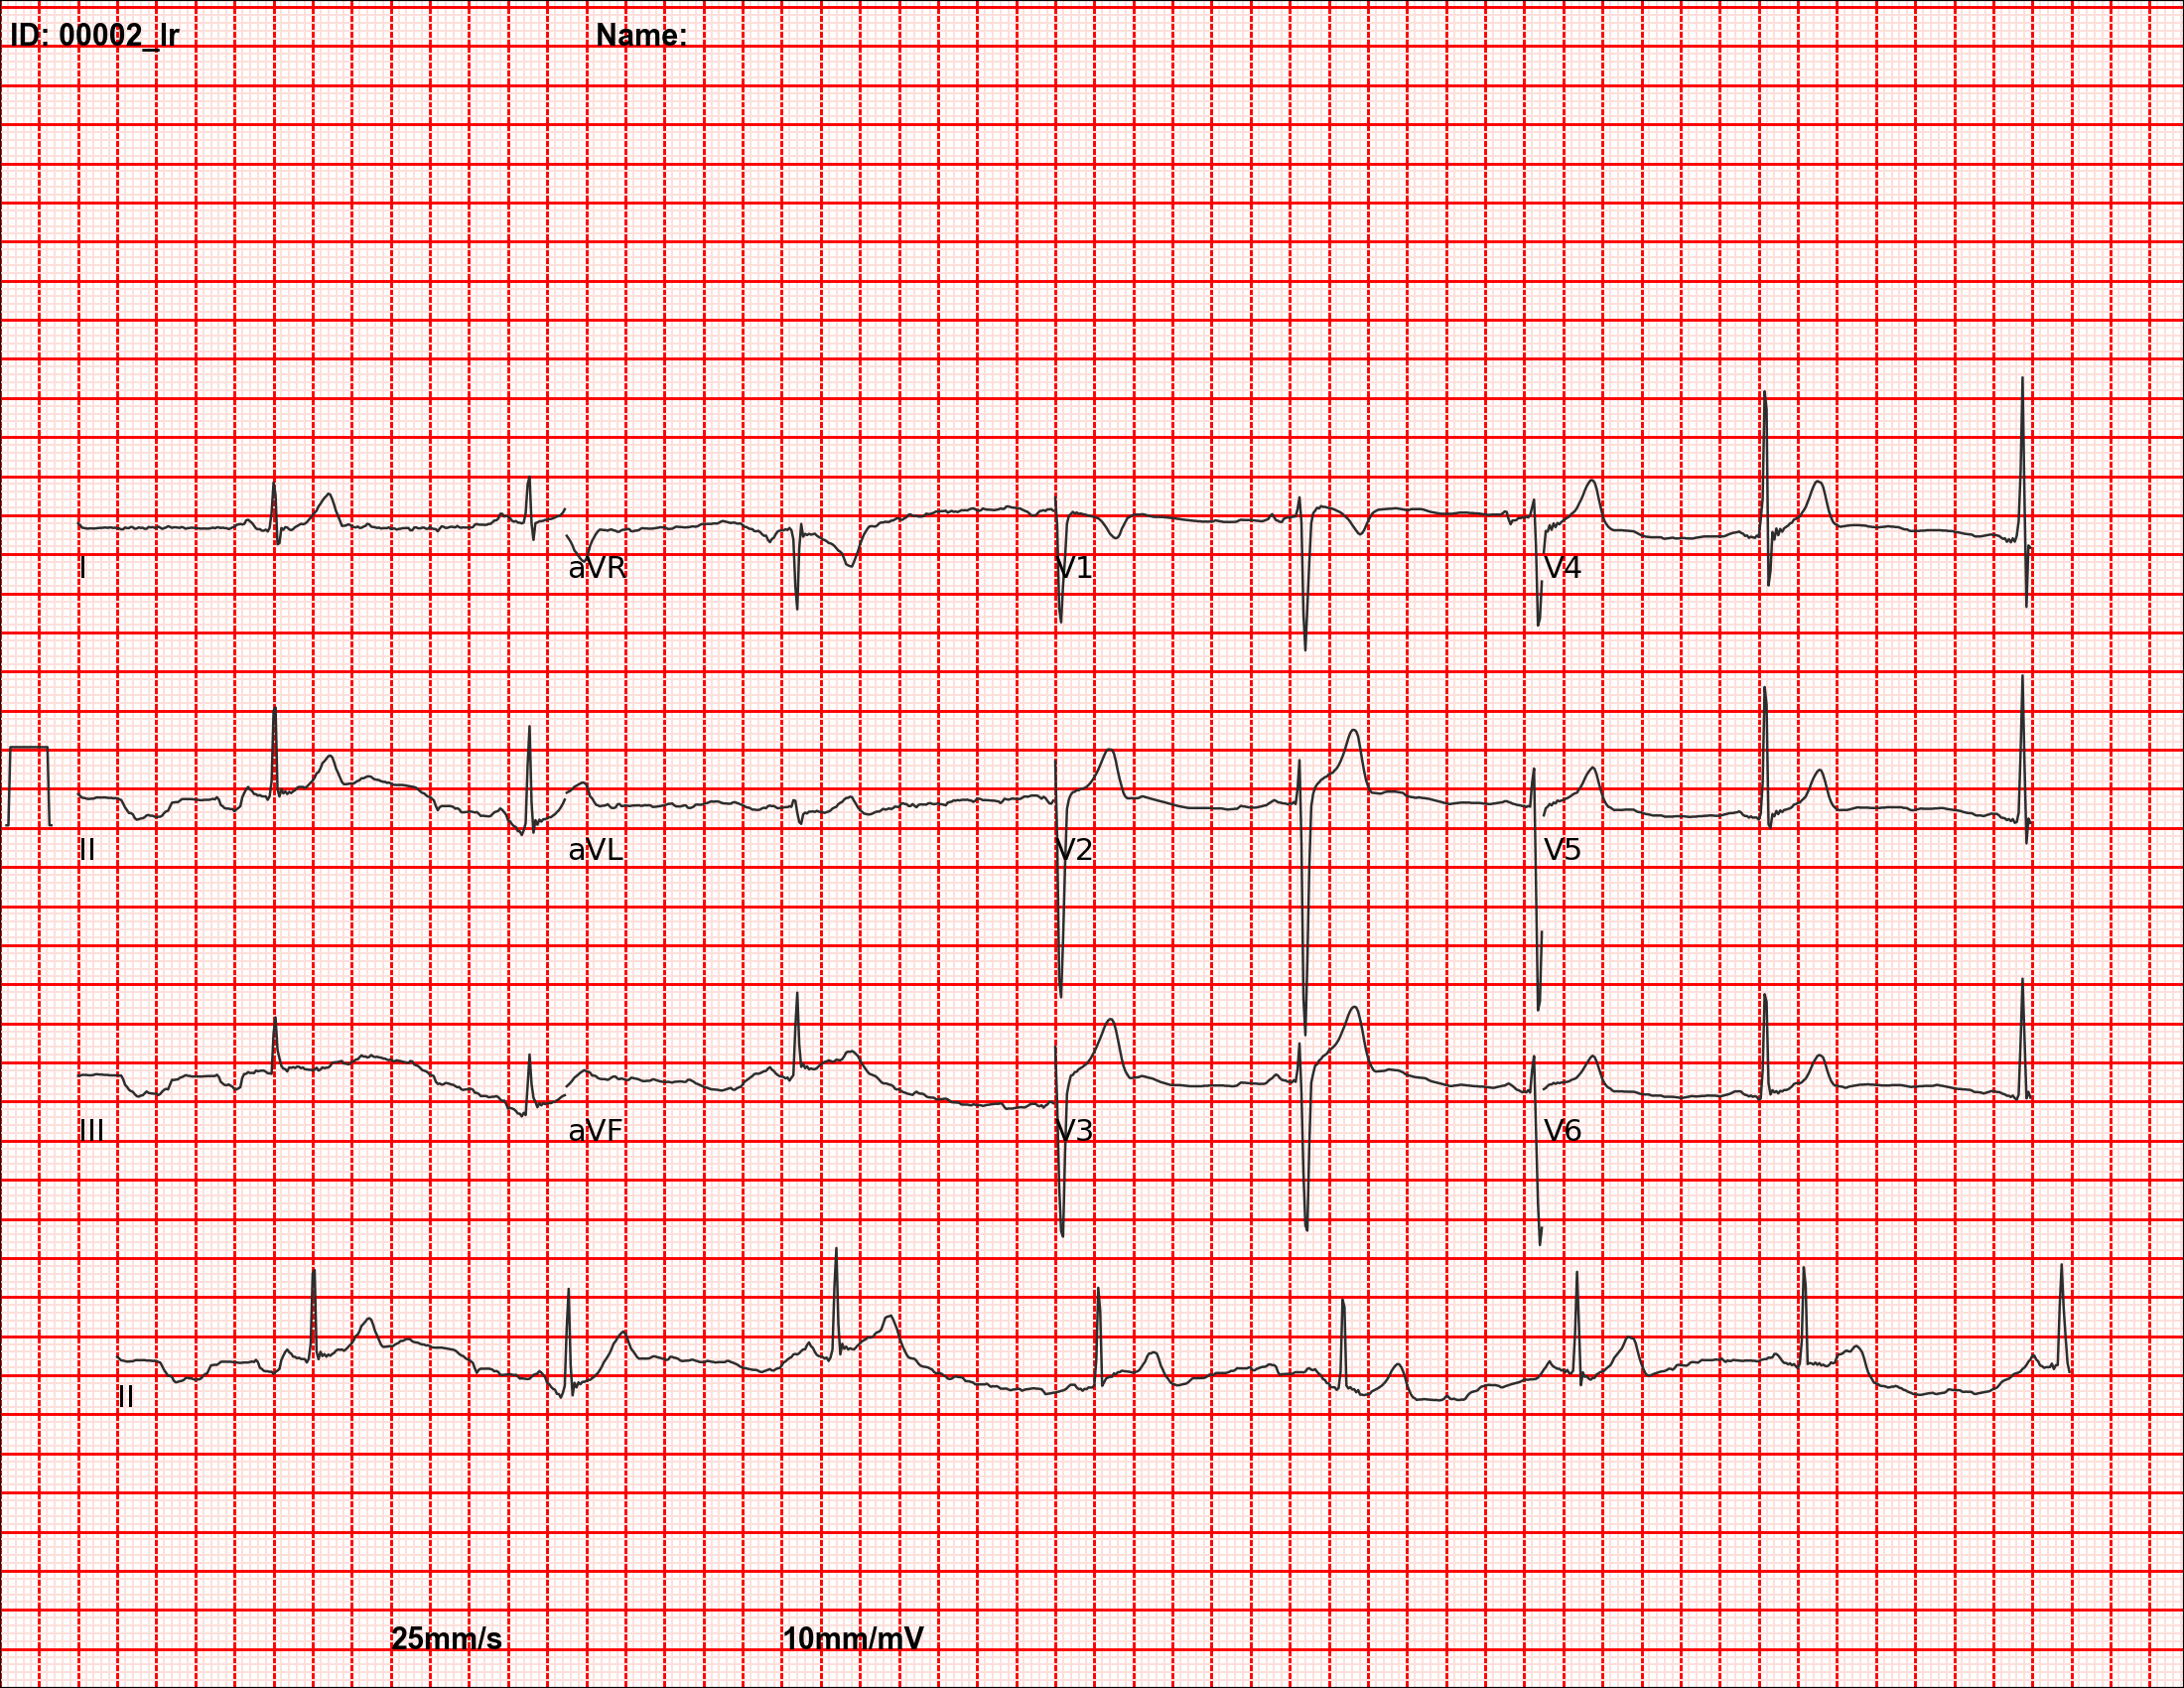
\includegraphics[width=\textwidth,height=5.3cm,keepaspectratio]{referto_clean.png}\\
      {\scriptsize Referto ECG su carta millimetrata (12 derivazioni).}
    \end{column}
  \end{columns}
\end{frame}

\begin{frame}{Lavori correlati: un gap aperto}
  \begin{itemize}
    \item La digitalizzazione degli ECG cartacei è già stata affrontata, ma gli approcci esistenti presentano limiti operativi:
    \begin{itemize}
      \item modelli con codice \alert{non funzionante} o non riproducibile (ECGtizer, Li et al., Wu et al.);
      \item strumenti \alert{instabili} su tracciati rumorosi o legati a processi manuali (ECGMiner, Fortune et al.);
      \item soluzioni \alert{a pagamento} o senza codice pubblicato.
    \end{itemize}
    \item \textbf{ECG-Image-Kit}: toolbox open-source per la generazione sintetica, ma non produce immagini sufficientemente \alert{degradate} per simulare le condizioni reali.
  \end{itemize}
  \vspace{2mm}
  \begin{block}{Contributo di questo lavoro}
    Una pipeline di generazione più controllata \textbf{e} un segmentatore addestrato specificamente su immagini con artefatti realistici.
  \end{block}
\end{frame}

\begin{frame}{Obiettivo: una pipeline a due stadi}
  \vfill
  \begin{columns}[T,onlytextwidth]
    \begin{column}{0.47\textwidth}
      \begin{block}{Stadio 1: Generazione sintetica}
        \begin{minipage}[t][1.9cm]{\linewidth}
          Dai segnali digitali a immagini ECG realistiche e \alert{degradate}, con \textbf{ground truth intrinseca} (la maschera del tracciato), senza alcuna annotazione manuale.
        \end{minipage}
      \end{block}
    \end{column}
    \hfill
    \begin{column}{0.47\textwidth}
      \begin{block}{Stadio 2: Segmentazione semantica}
        \begin{minipage}[t][1.9cm]{\linewidth}
          Una rete U-Net che \alert{isola il tracciato} del segnale da griglia, sfondo e artefatti, generalizzando anche ai documenti clinici degradati reali.
        \end{minipage}
      \end{block}
    \end{column}
  \end{columns}
  \vfill
  \begin{center}
    \footnotesize
    \fbox{Segnale digitale} $\rightarrow$ \fbox{Rendering} $\rightarrow$ \fbox{Artefatti} $\rightarrow$ \fbox{\textbf{Immagine + maschera}} $\rightarrow$ \fbox{Training U-Net}
  \end{center}
  \vfill
  \begin{center}\footnotesize\textit{La conversione finale maschera $\rightarrow$ segnale numerico è uno sviluppo futuro.}\end{center}
  \vfill
\end{frame}

\section{Stadio 1: Generazione Sintetica}

\begin{frame}{Dal segnale all'immagine: rendering calibrato}
  \begin{columns}[T]
    \begin{column}{0.5\textwidth}
      \begin{itemize}
        \item Rendering vettoriale con \texttt{Matplotlib}, calibrato sulla carta millimetrata clinica:
        \begin{itemize}
          \item \footnotesize asse $x$: 5\,mm $=0.2$\,s (25 mm/s)
          \item \footnotesize asse $y$: 5\,mm $=0.5$\,mV (10 mm/mV)
        \end{itemize}
        \item Corrispondenza \alert{millimetrica} pixel $\leftrightarrow$ grandezze fisiche.
        \item 4 layout clinici ($12\times1$, $6\times2$, $3\times4$, $6\times1$ split) con segmentazione temporale coerente.
        \item Estensioni al rendering: supporto \textbf{CODE-15\%} (HDF5), configurazione via YAML, rendering \alert{in-memory}.
      \end{itemize}
    \end{column}
    \begin{column}{0.5\textwidth}
      \centering
      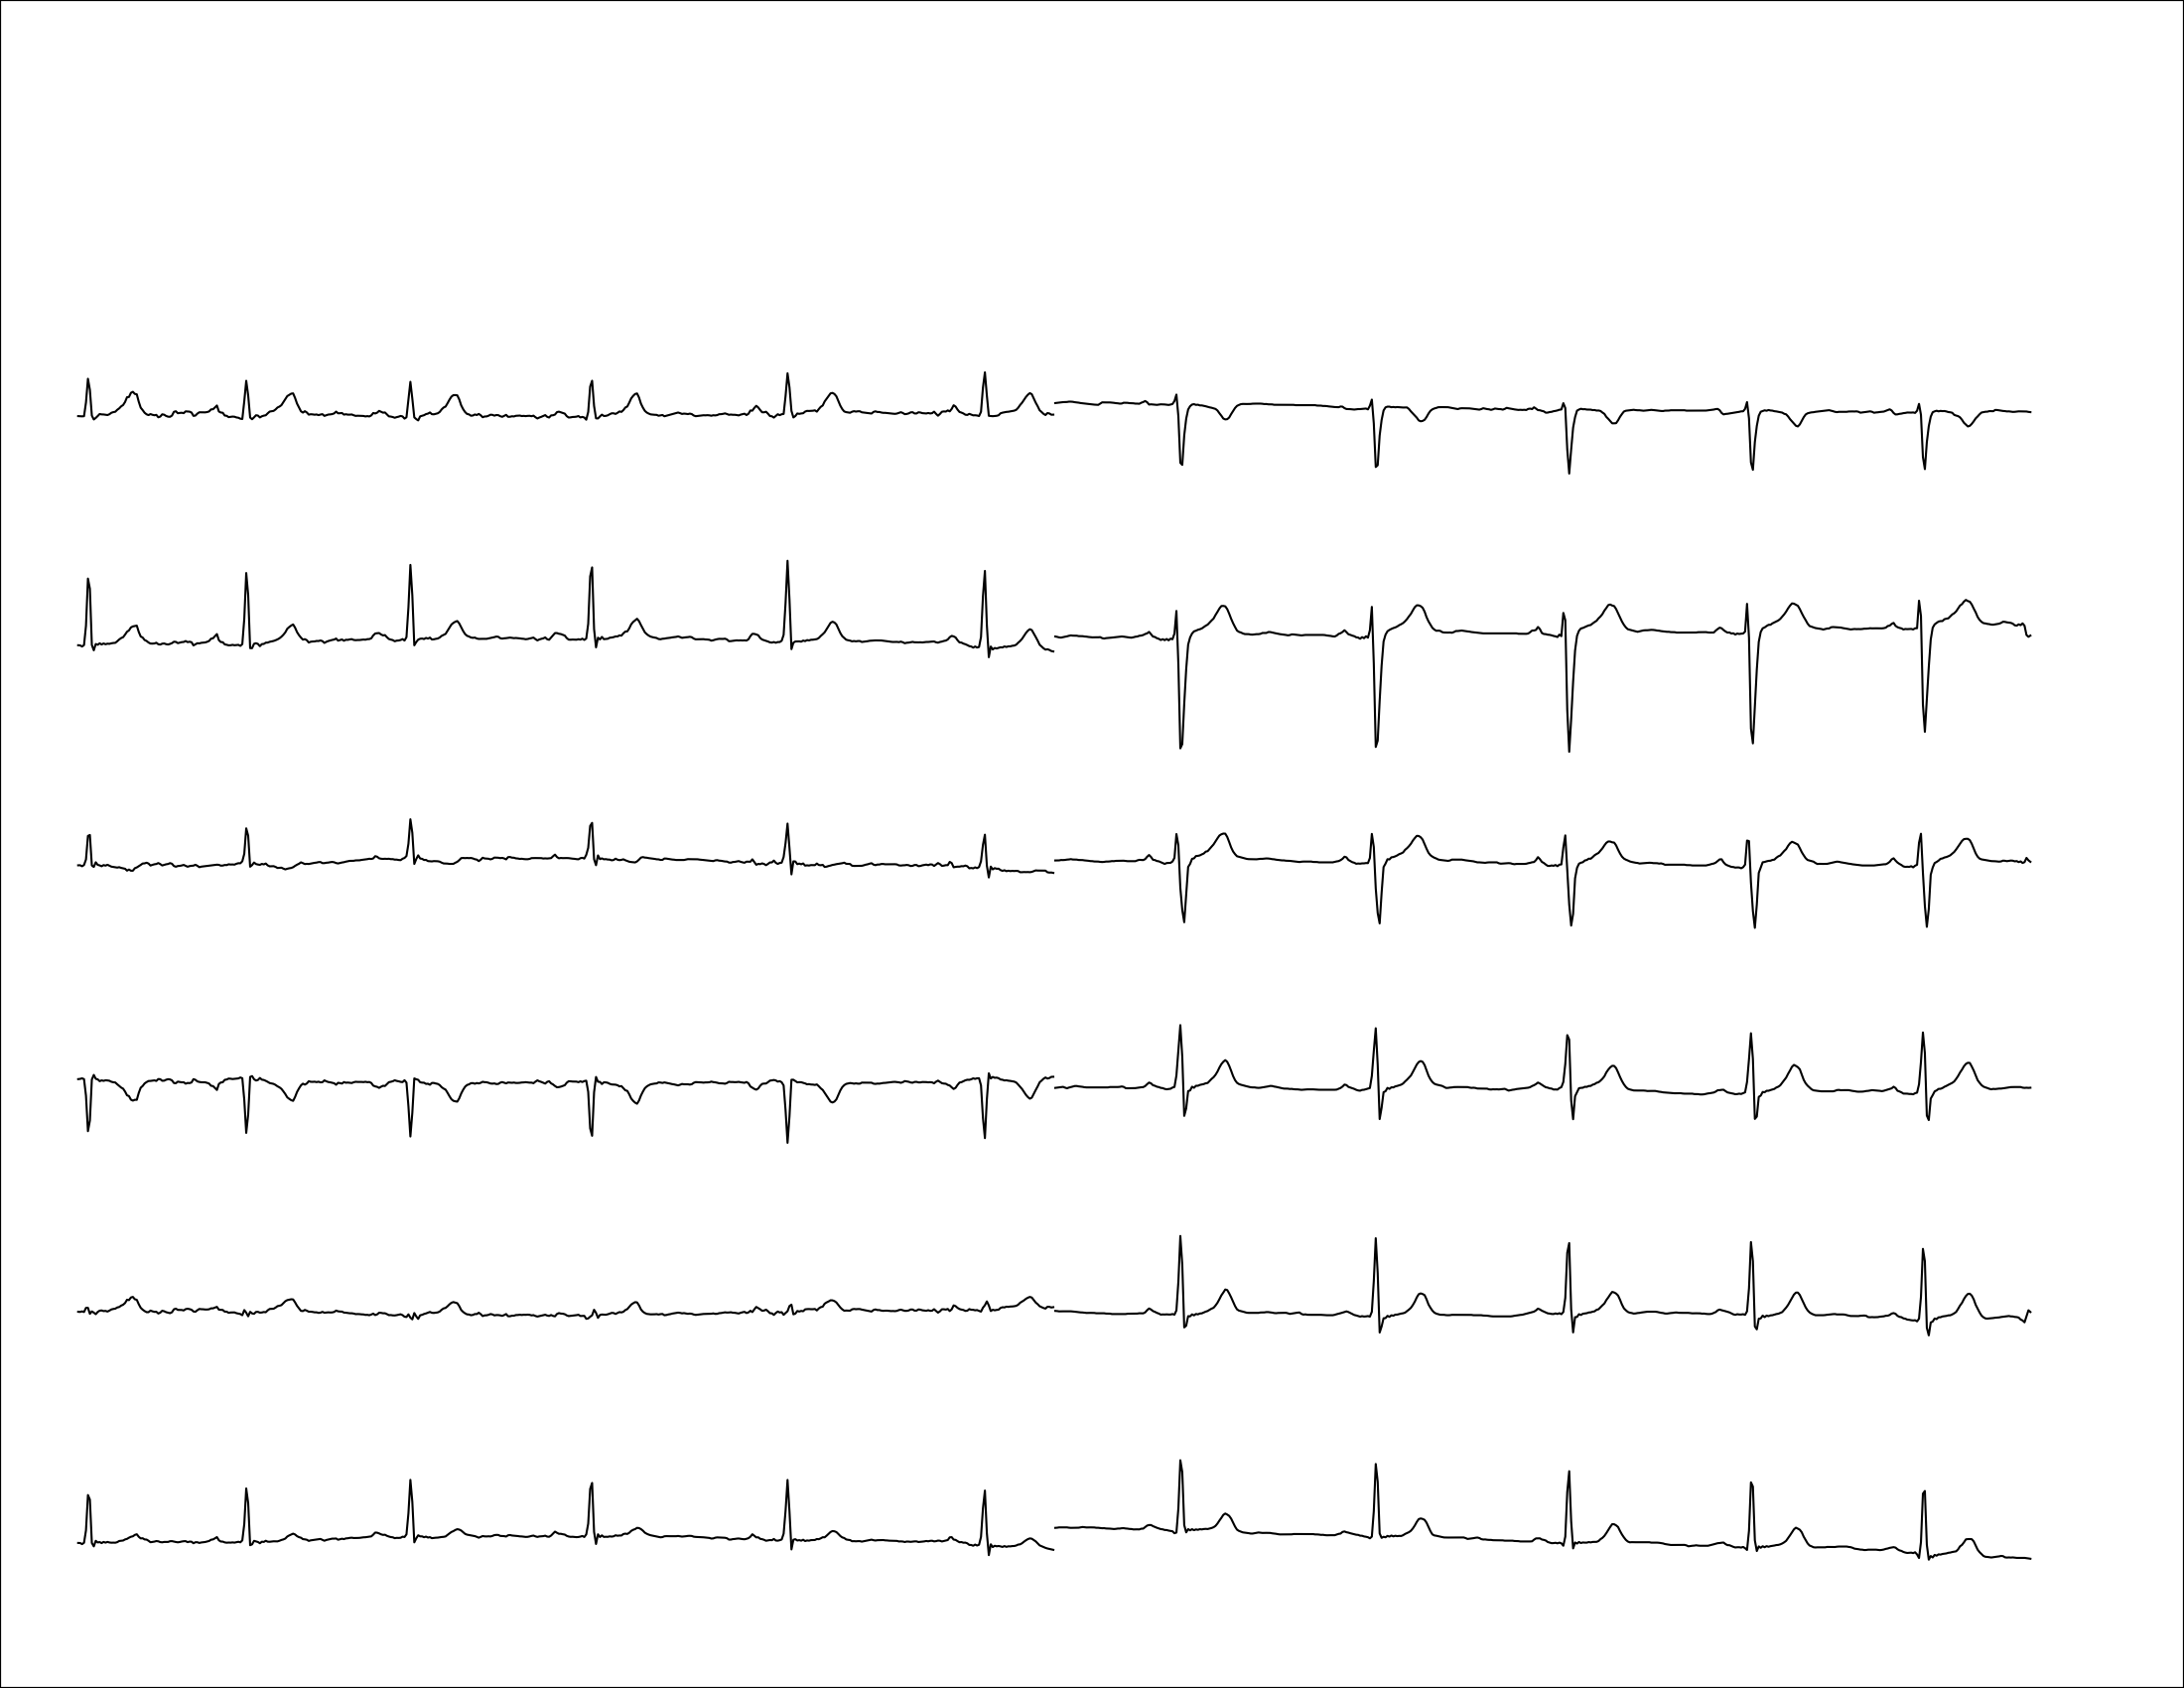
\includegraphics[width=0.92\textwidth]{clean_plot.png}\\
      {\scriptsize Tracciato vettoriale pulito su canvas calibrato.}
    \end{column}
  \end{columns}
\end{frame}

\begin{frame}{Il \emph{domain gap}: artefatti realistici e contributi originali}
  \begin{columns}[T]
    \begin{column}{0.5\textwidth}
      \footnotesize
      Modelli addestrati su immagini \alert{pulite} crollano su documenti reali, pieni di difetti accumulati nel ciclo di vita del documento.
      \vspace{1mm}
      \begin{block}{Tre classi di artefatti}
        \footnotesize
        \begin{itemize}
          \item \textbf{Testo manoscritto} (RNN+MDN, NLP biomedico)
          \item \textbf{Pieghe e rugosità} (image quilting + min-cut)
          \item \textbf{Degradazione foto/geometrica}: rotazione e rumore gaussiano (base) + \alert{blur, sale-pepe, JPEG, luminosità, dropout} introdotti
        \end{itemize}
      \end{block}
      \textbf{Estensioni introdotte:} dropout \alert{differenziale} (tracciato vs sfondo), shift geometrico per elemento, \textbf{generazione maschera (\textit{ground truth})}, bounding box orientati, supporto CODE-15\%.
    \end{column}
    \begin{column}{0.5\textwidth}
      \centering
      \begin{tabular}{cc}
        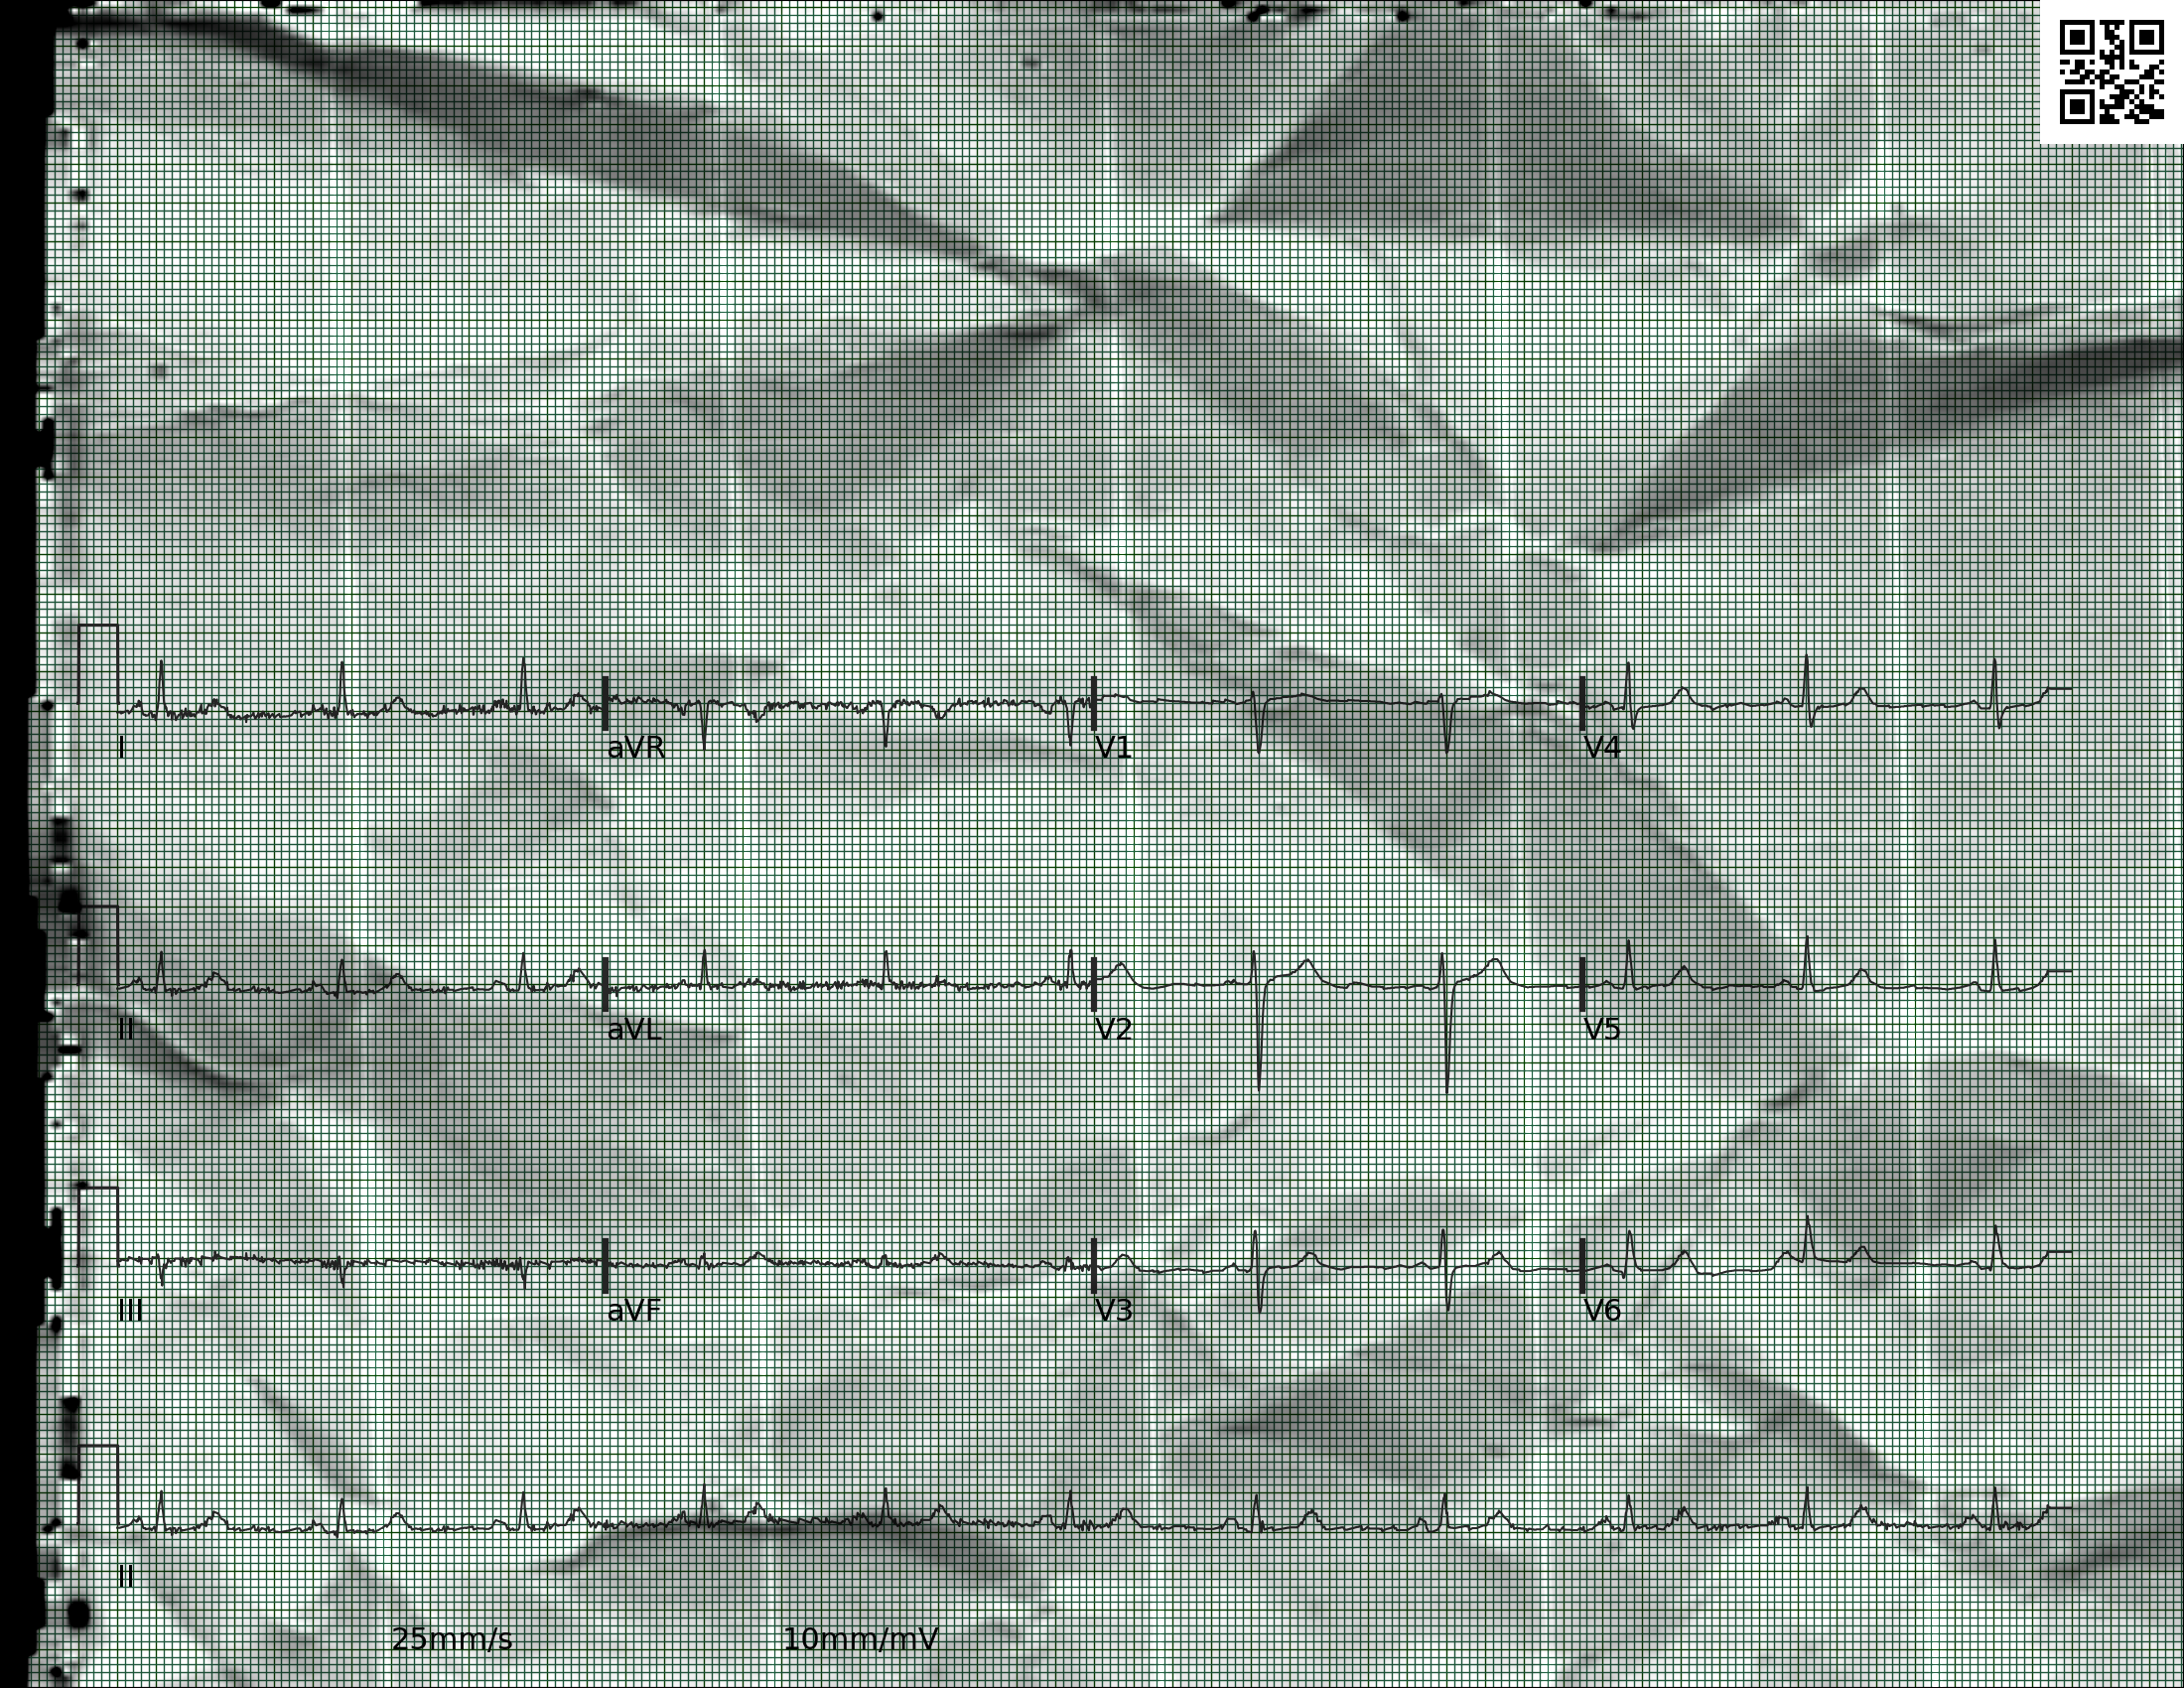
\includegraphics[width=0.46\textwidth,height=2.4cm,keepaspectratio]{sample_wrinkles.png} &
        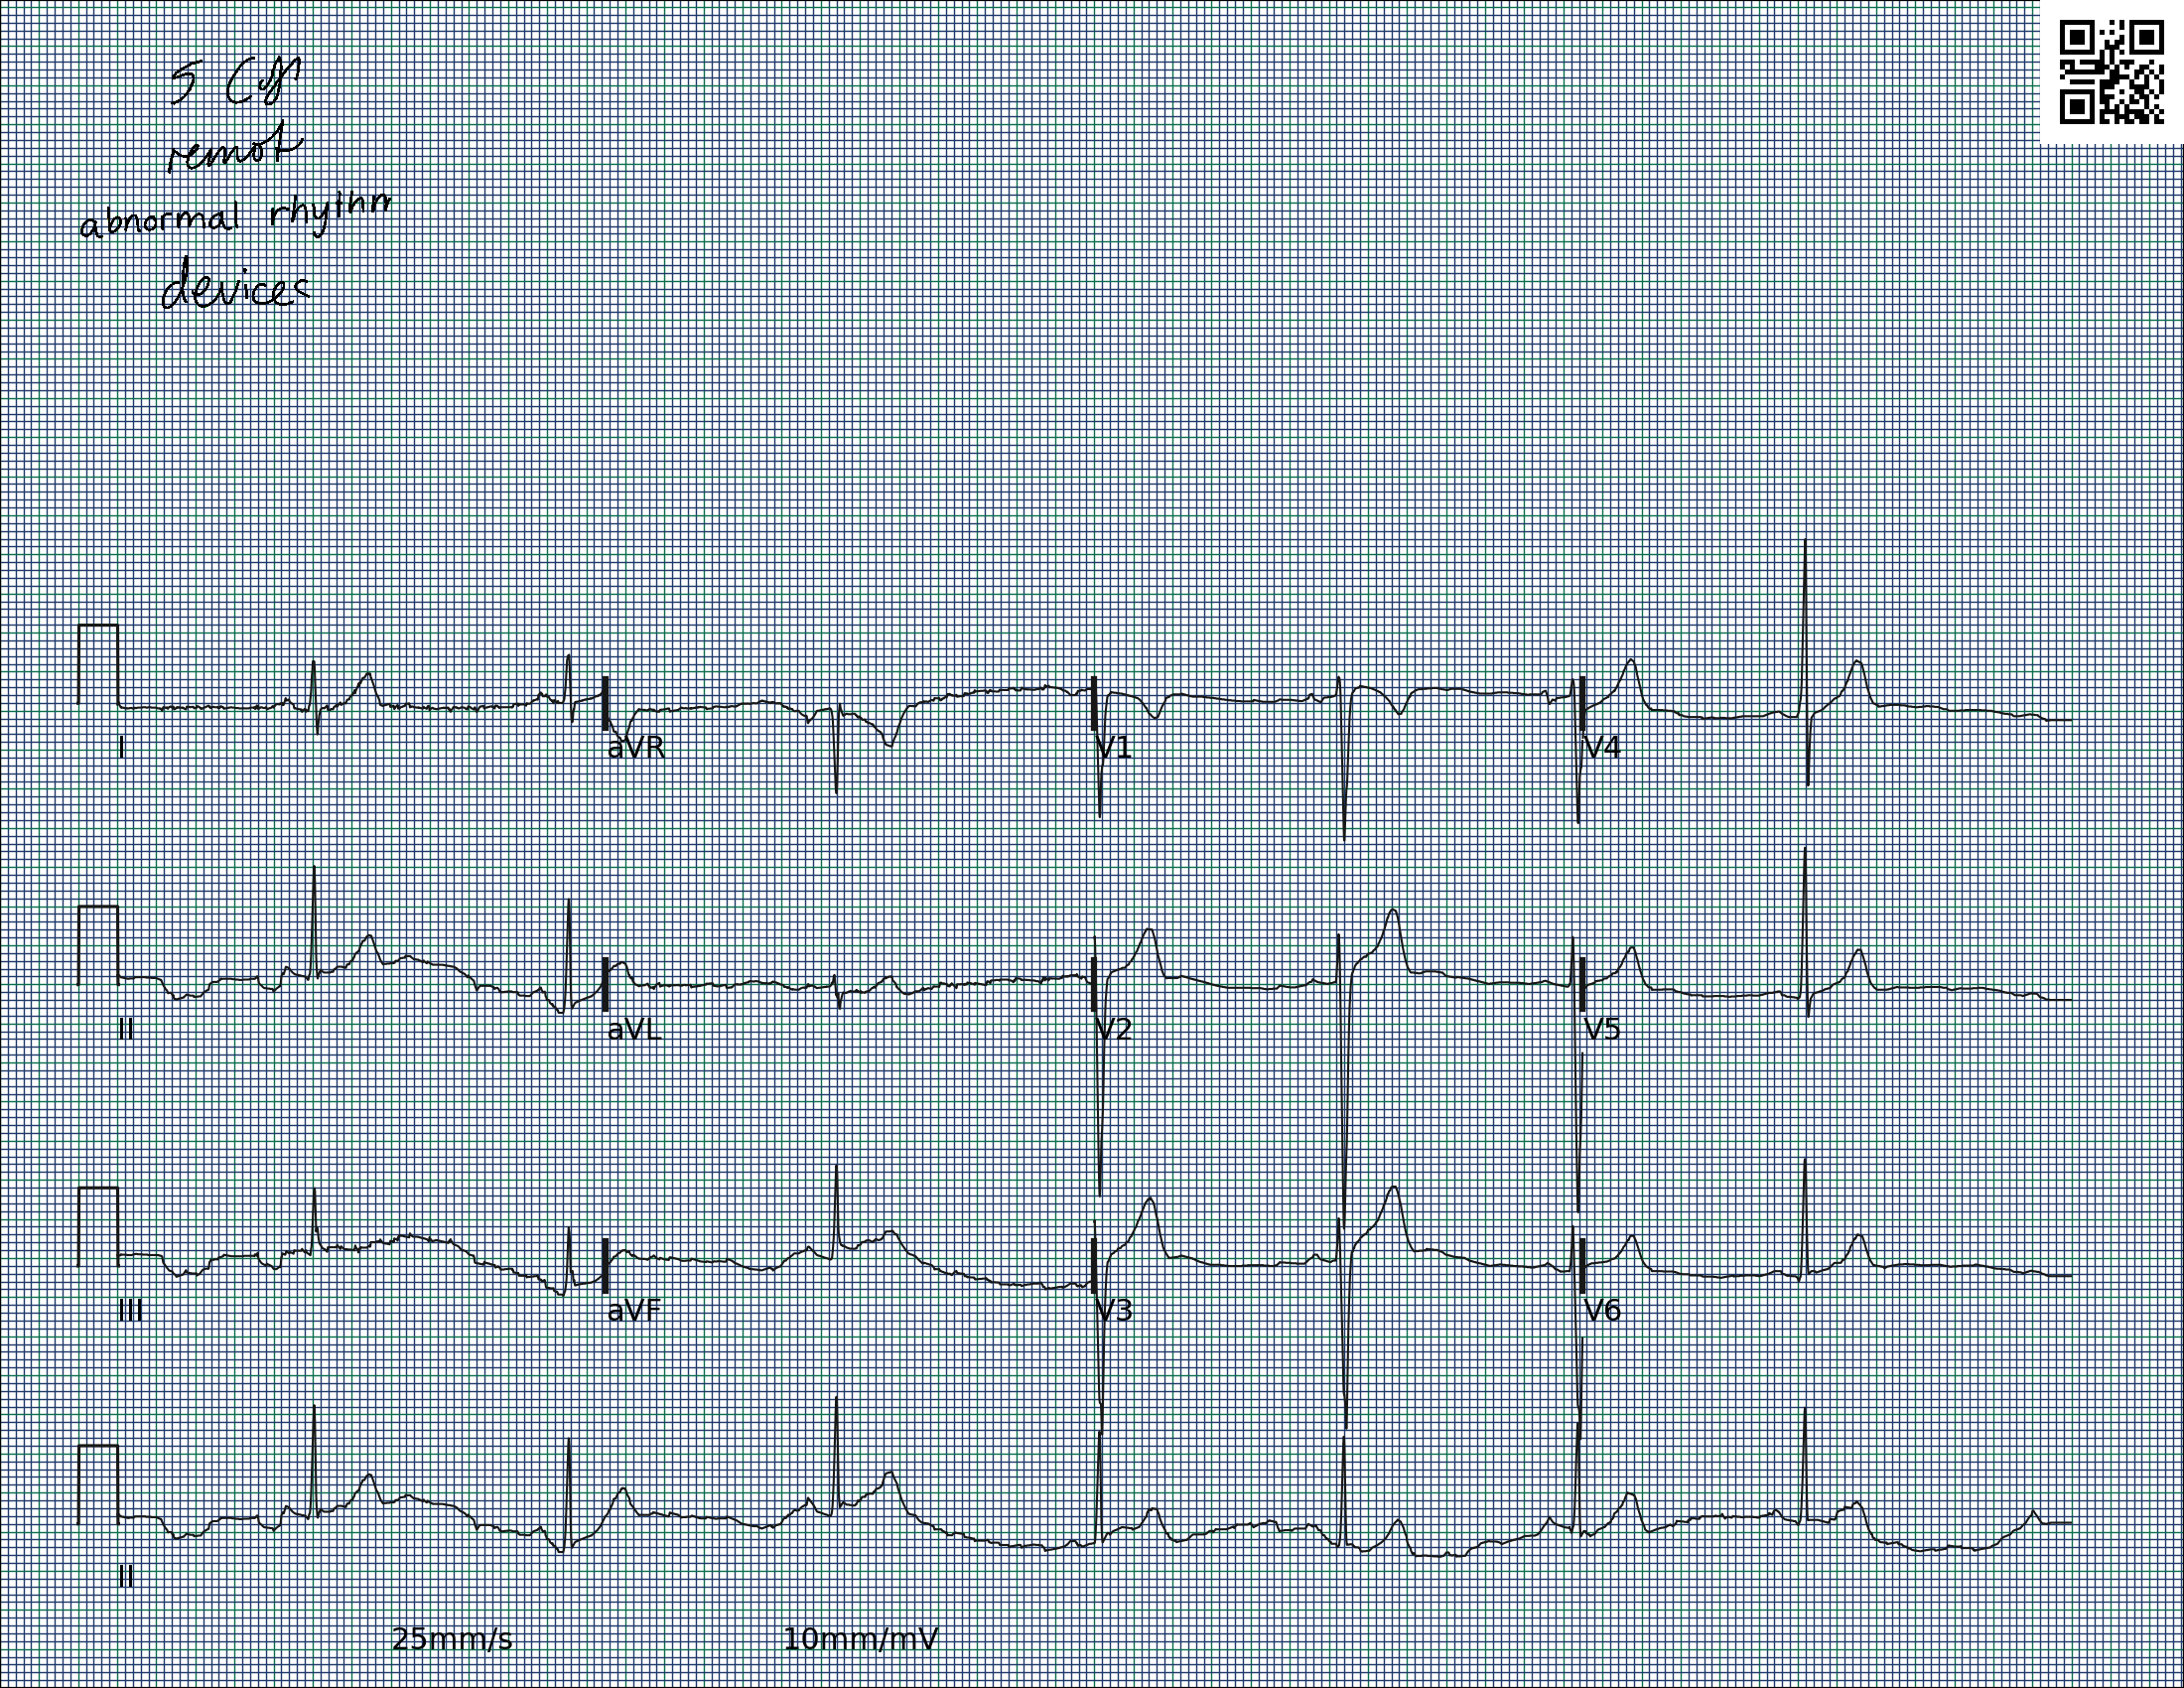
\includegraphics[width=0.46\textwidth,height=2.4cm,keepaspectratio]{sample_hwtext.png} \\
        {\scriptsize Pieghe e rugosità} & {\scriptsize Testo manoscritto} \\[1mm]
        \multicolumn{2}{c}{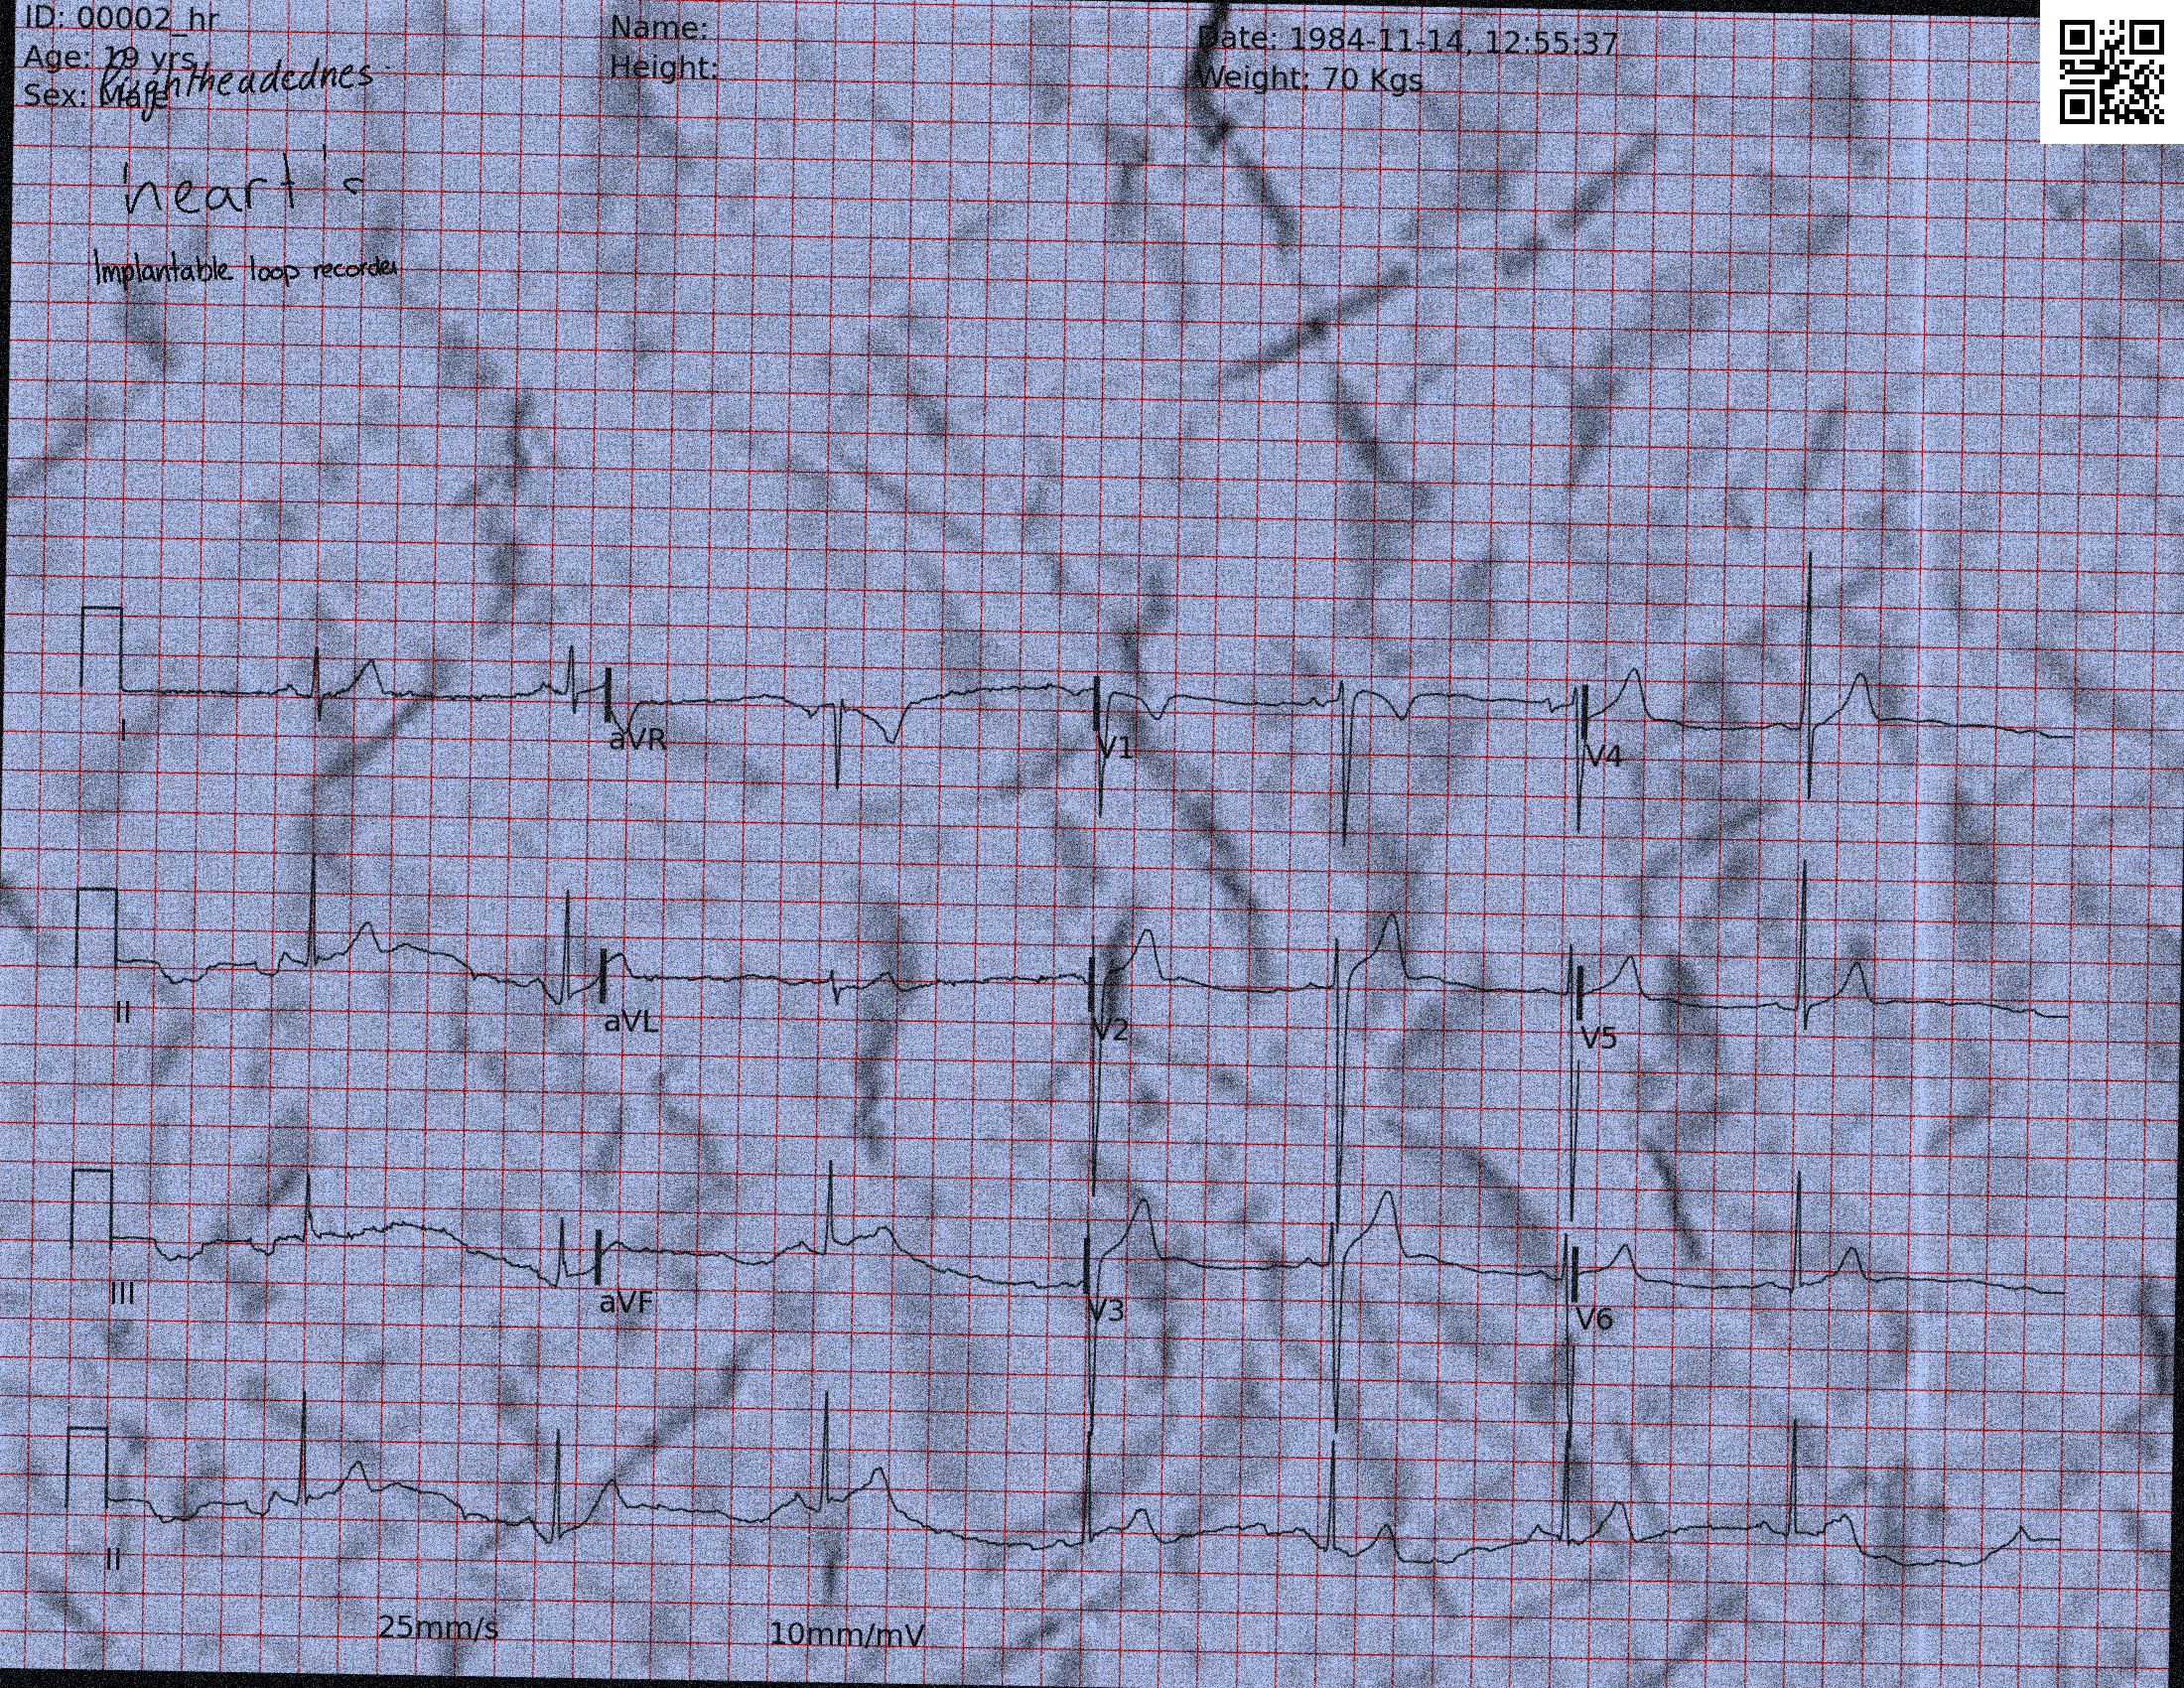
\includegraphics[width=0.6\textwidth,height=2.7cm,keepaspectratio]{sample_all_artifacts.png}} \\
        \multicolumn{2}{c}{\scriptsize Configurazione completa combinata}
      \end{tabular}
    \end{column}
  \end{columns}
\end{frame}

\begin{frame}{Coppia immagine / maschera: ground truth gratuita}
  \begin{columns}[c]
    \begin{column}{0.5\textwidth}
      \centering
      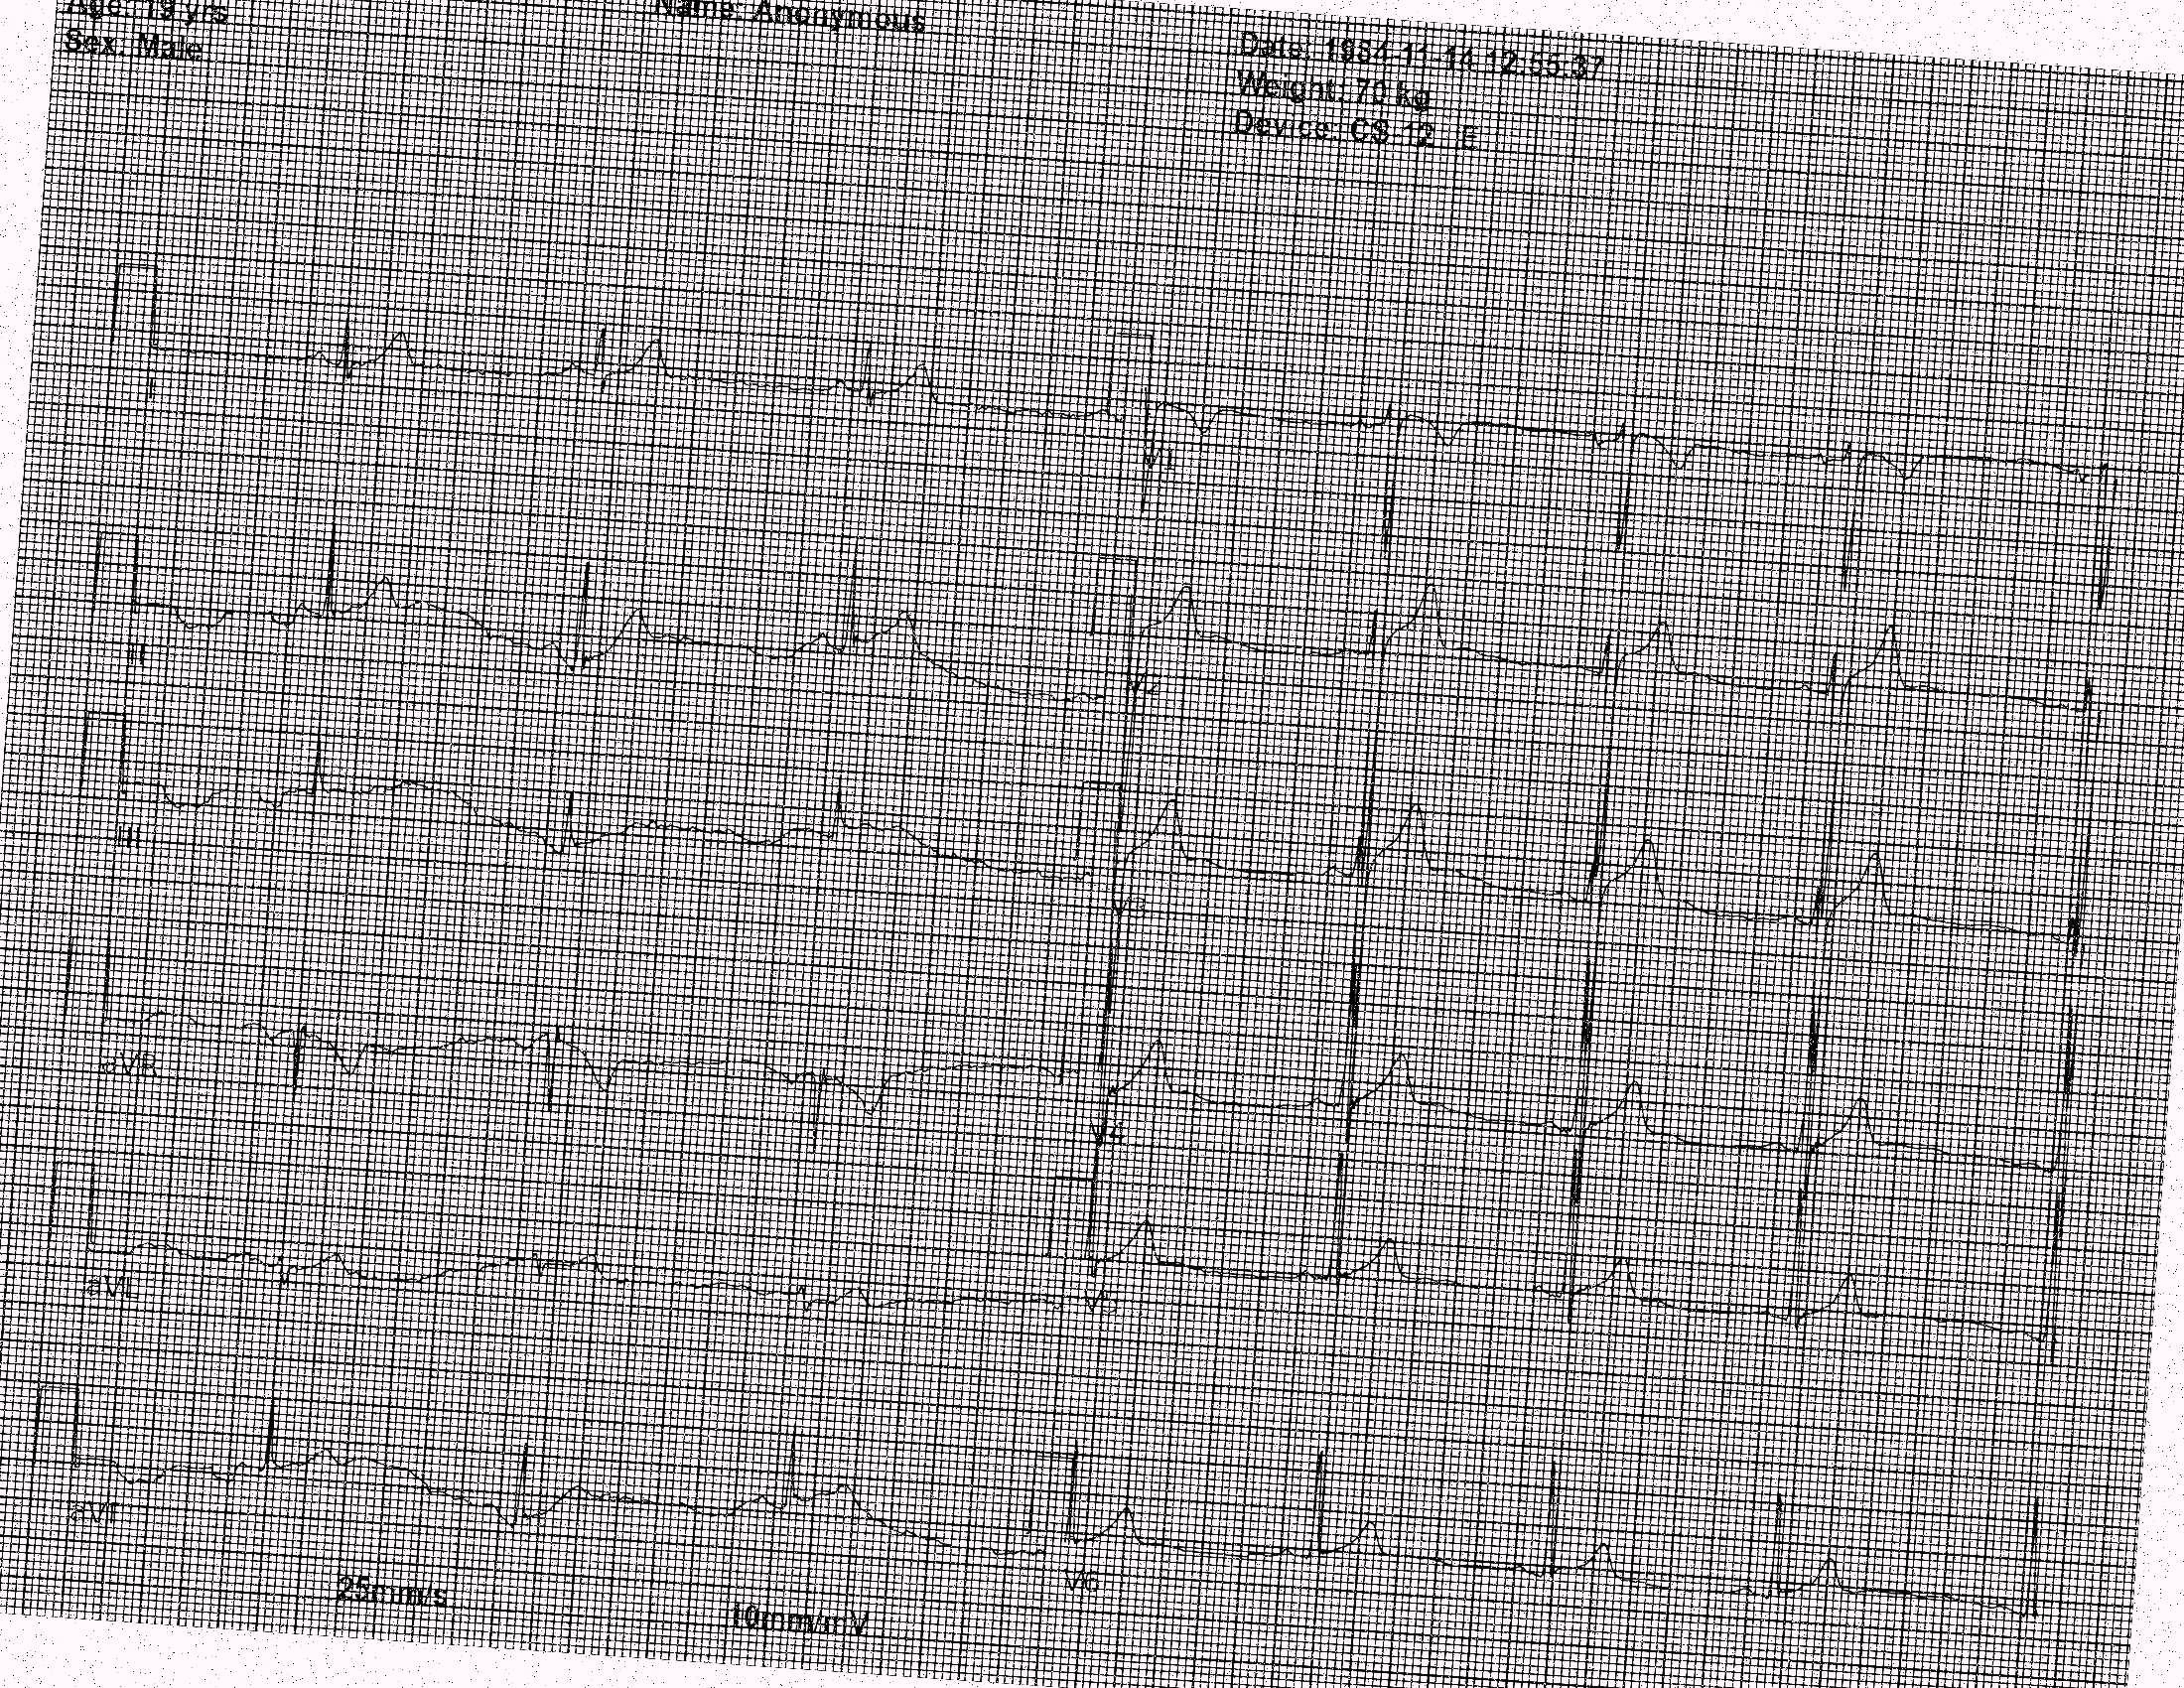
\includegraphics[width=0.95\textwidth,height=5.2cm,keepaspectratio]{00002_lr-0.png}\\
      {\scriptsize Immagine sintetica (input del modello)}
    \end{column}
    \begin{column}{0.5\textwidth}
      \centering
      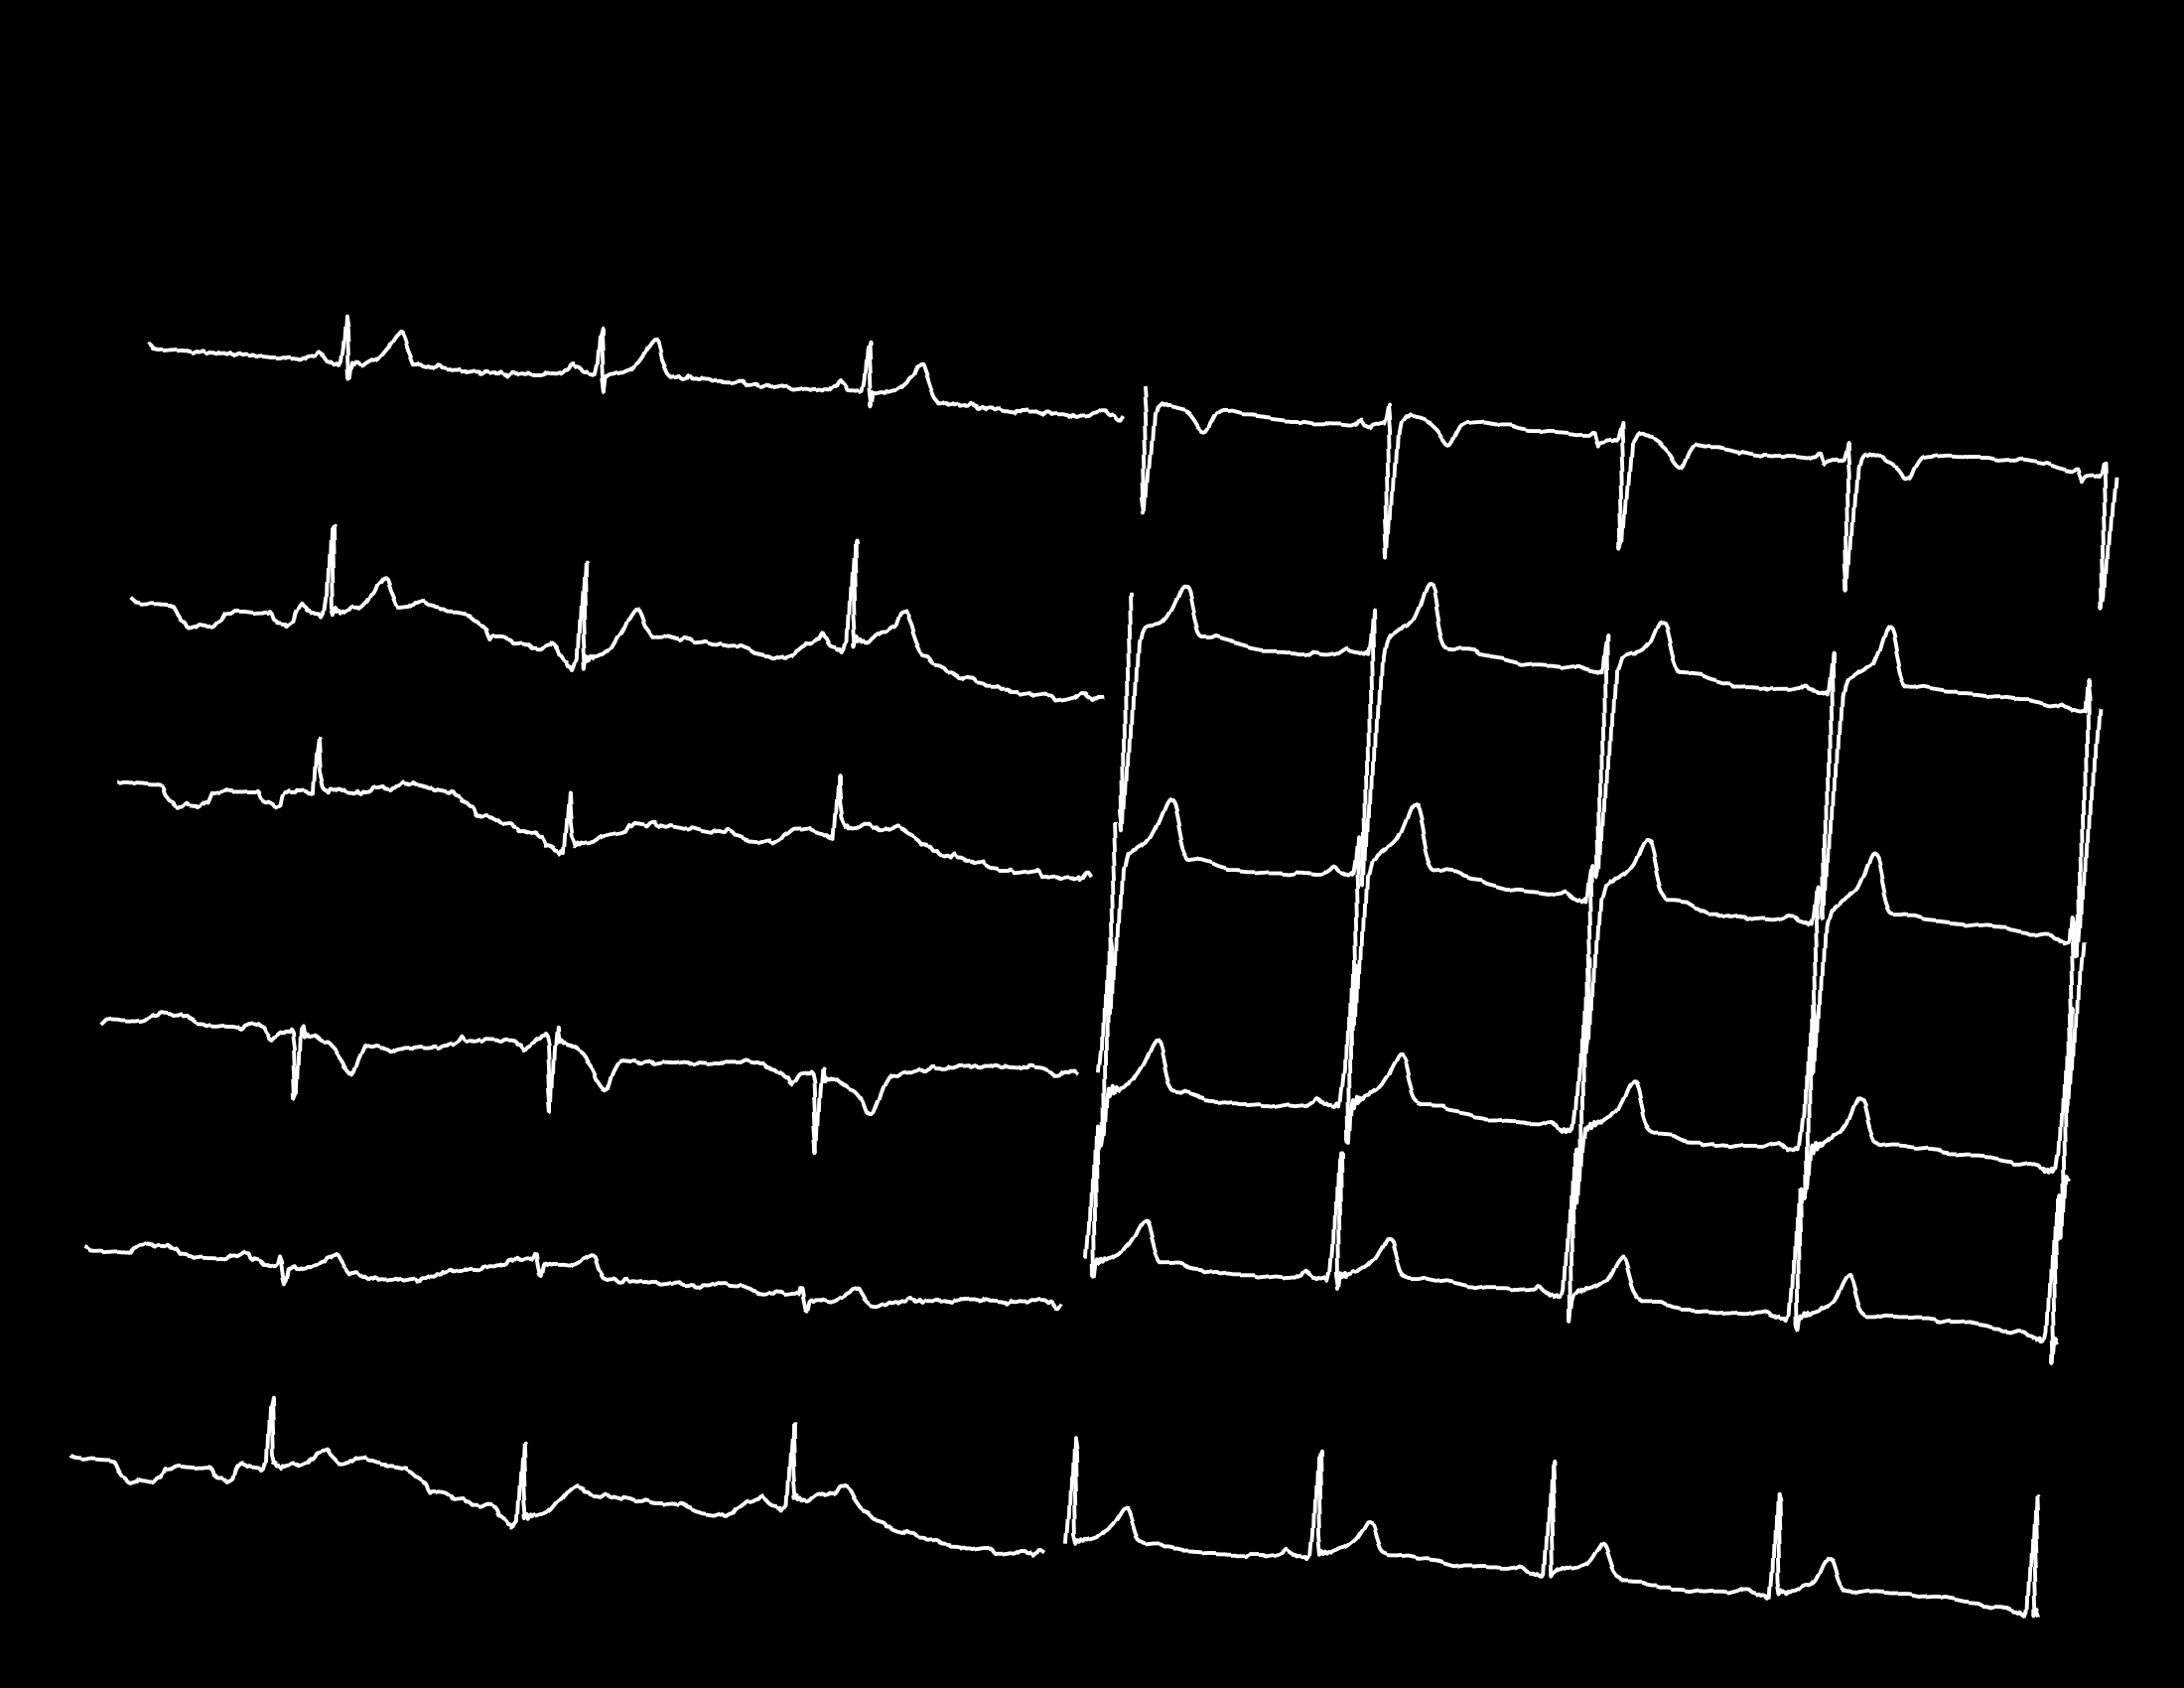
\includegraphics[width=0.95\textwidth,height=5.2cm,keepaspectratio]{00002_lr-0_clean.png}\\
      {\scriptsize Maschera binaria (ground truth)}
    \end{column}
  \end{columns}
  \vspace{2mm}
  \begin{center}
    Le stesse trasformazioni geometriche sono applicate a entrambe $\Rightarrow$ corrispondenza \alert{pixel-per-pixel}.
  \end{center}
\end{frame}

\begin{frame}{Risultati Stadio 1: parallelizzazione}
  \begin{columns}[T]
    \begin{column}{0.46\textwidth}
      \begin{itemize}
        \item Carico \alert{\emph{embarrassingly parallel}}: ogni ECG è indipendente.
        \item \texttt{ProcessPoolExecutor} aggira il GIL di Python (vero parallelismo multi-core).
        \item Speedup massimo $\mathbf{3.03\times}$ a \textbf{8 worker} (= core fisici).
        \item Oltre non scala: carico \alert{CPU-bound}, non I/O-bound $\Rightarrow$ l'hyperthreading non aiuta (più banda di memoria satura).
        \item Su PTB-XL (>21\,000 record) i tempi di generazione si riducono drasticamente.
      \end{itemize}
    \end{column}
    \begin{column}{0.54\textwidth}
      \centering
      \begin{tikzpicture}
      \begin{axis}[
          width=\textwidth, height=5.2cm,
          xlabel={Numero di processi}, ylabel={Speedup},
          ymin=0, ymax=4.2, xtick={1,2,4,8,16}, ytick={0,1,2,3,4},
          legend style={at={(0.97,0.03)}, anchor=south east, font=\scriptsize},
          mark size=2pt, grid=major, grid style={gray!20},
      ]
      \addplot[color=accent, mark=*, thick] coordinates {(1,1.00)(2,1.77)(4,2.74)(8,3.03)(16,2.47)};
      \addlegendentry{Speedup reale}
      \addplot[color=gray, dashed, thin] coordinates {(1,1)(16,16)};
      \addlegendentry{Ideale}
      \end{axis}
      \end{tikzpicture}\\
      {\scriptsize Speedup vs numero di processi (baseline, 32 immagini).}
    \end{column}
  \end{columns}
\end{frame}

\section{Stadio 2: Segmentazione Semantica}

\begin{frame}{Architettura: U-Net + attenzione scSE}
  \begin{columns}[T]
    \begin{column}{0.55\textwidth}
      \begin{itemize}
        \item \textbf{U-Net} encoder-decoder con \alert{skip connection}: recupera i dettagli spaziali fini dei tracciati sottili.
        \item Encoder \texttt{resnet50} pre-addestrato su ImageNet (intercambiabile: EfficientNet, transformer MiT).
        \item Decoder con attenzione \alert{scSE}: ricalibra le feature per \textit{canale} (cSE) e per \textit{posizione} (sSE).
        \item Riduce i falsi positivi sulla griglia millimetrata, che condivide tratti visivi col tracciato.
      \end{itemize}
    \end{column}
    \begin{column}{0.45\textwidth}
      \centering
      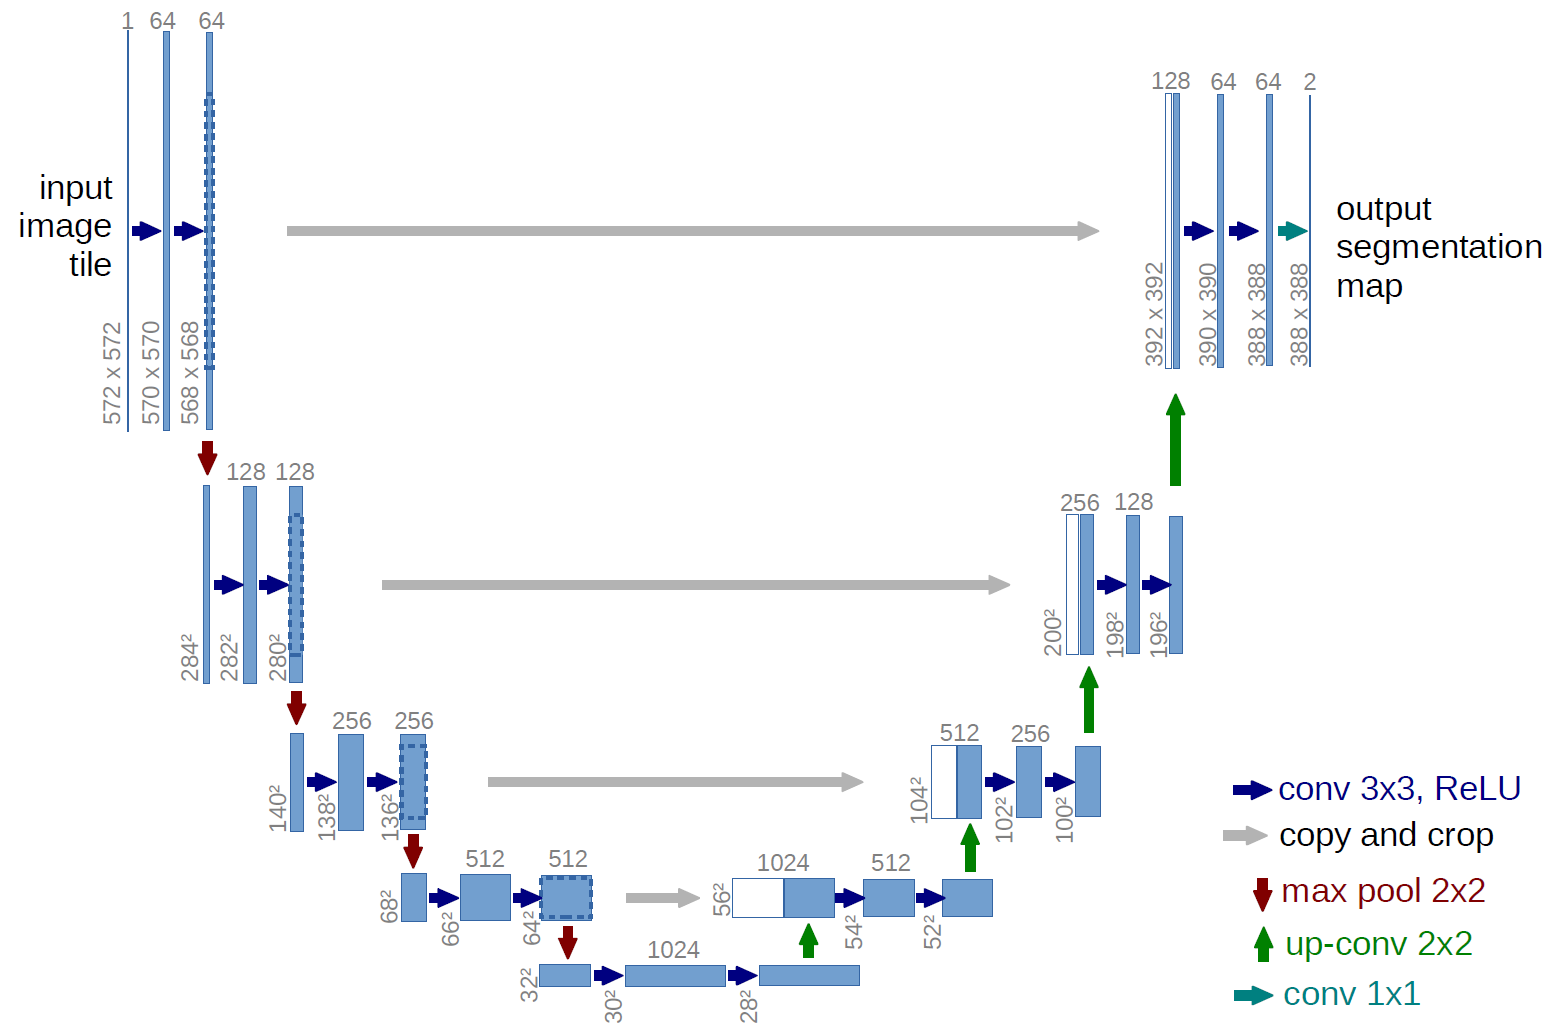
\includegraphics[width=\textwidth,height=3.4cm,keepaspectratio]{u-net-architecture.png}\\[1mm]
      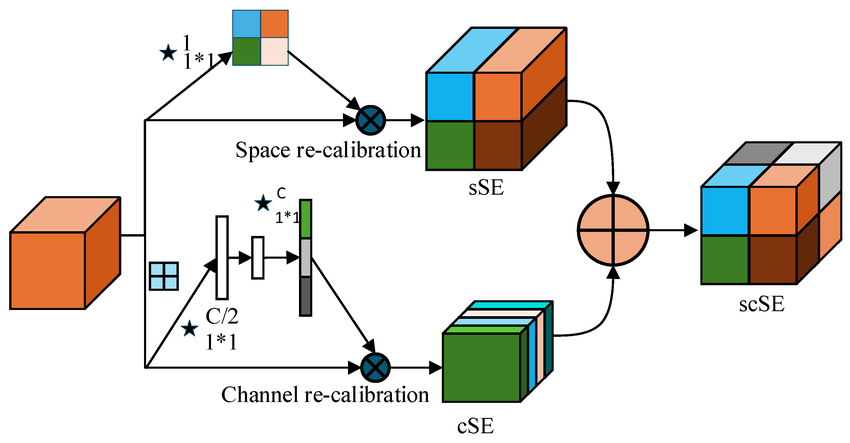
\includegraphics[width=0.8\textwidth,height=2.4cm,keepaspectratio]{scSE.png}\\
      {\scriptsize U-Net (alto) e blocco scSE (basso).}
    \end{column}
  \end{columns}
\end{frame}

\begin{frame}{Funzione di perdita composita}
  \[
    \mathcal{L} = w_{\text{focal}}\,\mathcal{L}_{\text{Focal}}
                + w_{\text{dice}}\,\mathcal{L}_{\text{Dice}}
                + w_{\text{cl}}\,\mathcal{L}_{\text{clDice}}
  \]
  \vspace{1mm}
  \begin{columns}[T,onlytextwidth]
    \begin{column}{0.31\textwidth}
      \begin{block}{Focal}
        \begin{minipage}[t][2.2cm]{\linewidth}
          \footnotesize Gestisce lo \alert{sbilanciamento estremo} (<5\% pixel di tracciato): pesa di più i pixel difficili.
        \end{minipage}
      \end{block}
    \end{column}
    \hfill
    \begin{column}{0.31\textwidth}
      \begin{block}{Dice}
        \begin{minipage}[t][2.2cm]{\linewidth}
          \footnotesize Misura la \alert{sovrapposizione globale} maschera/ground truth; insensibile allo sbilanciamento.
        \end{minipage}
      \end{block}
    \end{column}
    \hfill
    \begin{column}{0.31\textwidth}
      \begin{block}{clDice}
        \begin{minipage}[t][2.2cm]{\linewidth}
          \footnotesize Confronta gli \alert{scheletri}: penalizza le \textbf{interruzioni topologiche} del tracciato (soft-skeleton differenziabile).
        \end{minipage}
      \end{block}
    \end{column}
  \end{columns}
  \vspace{2mm}
  \begin{center}
    \footnotesize Il peso della clDice \alert{cresce} con la difficoltà degli stage del curriculum.
  \end{center}
\end{frame}

\begin{frame}{Curriculum learning: dal facile al difficile}
  \begin{columns}[c]
    \begin{column}{0.52\textwidth}
      \begin{itemize}
        \item Tre stage di difficoltà crescente, \alert{senza reinizializzare} il modello:
        \begin{enumerate}
          \item \texttt{stage0\_easy}: immagini pulite
          \item \texttt{stage1\_medium}: degradazioni moderate
          \item \texttt{stage2\_hard}: campioni complessi
        \end{enumerate}
        \item \textbf{Unfreezing progressivo} dell'encoder + dropout crescente per stage.
        \item Learning rate decrescente ($10^{-4}\!\to\!10^{-6}$) contro il \textit{catastrophic forgetting}.
        \item Evita minimi locali dominati dagli esempi più rumorosi.
      \end{itemize}
    \end{column}
    \begin{column}{0.48\textwidth}
      \centering
      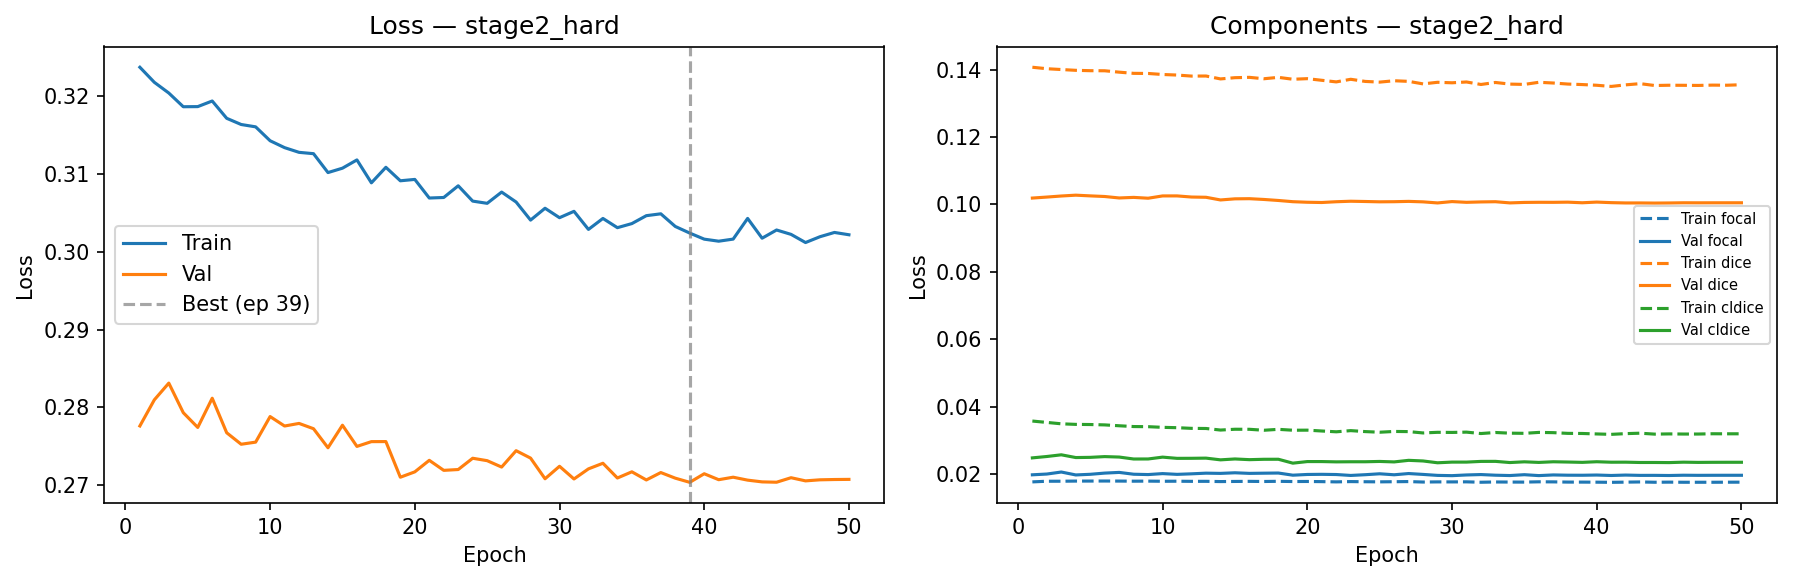
\includegraphics[width=\textwidth]{loss_stage2_hard.png}\\
      {\scriptsize Diagnostica dello \texttt{stage2\_hard}: loss totale e componenti.}
    \end{column}
  \end{columns}
\end{frame}

\begin{frame}{Risultati Stadio 2: effetto del curriculum}
  \begin{columns}[c]
    \begin{column}{0.5\textwidth}
      \centering
      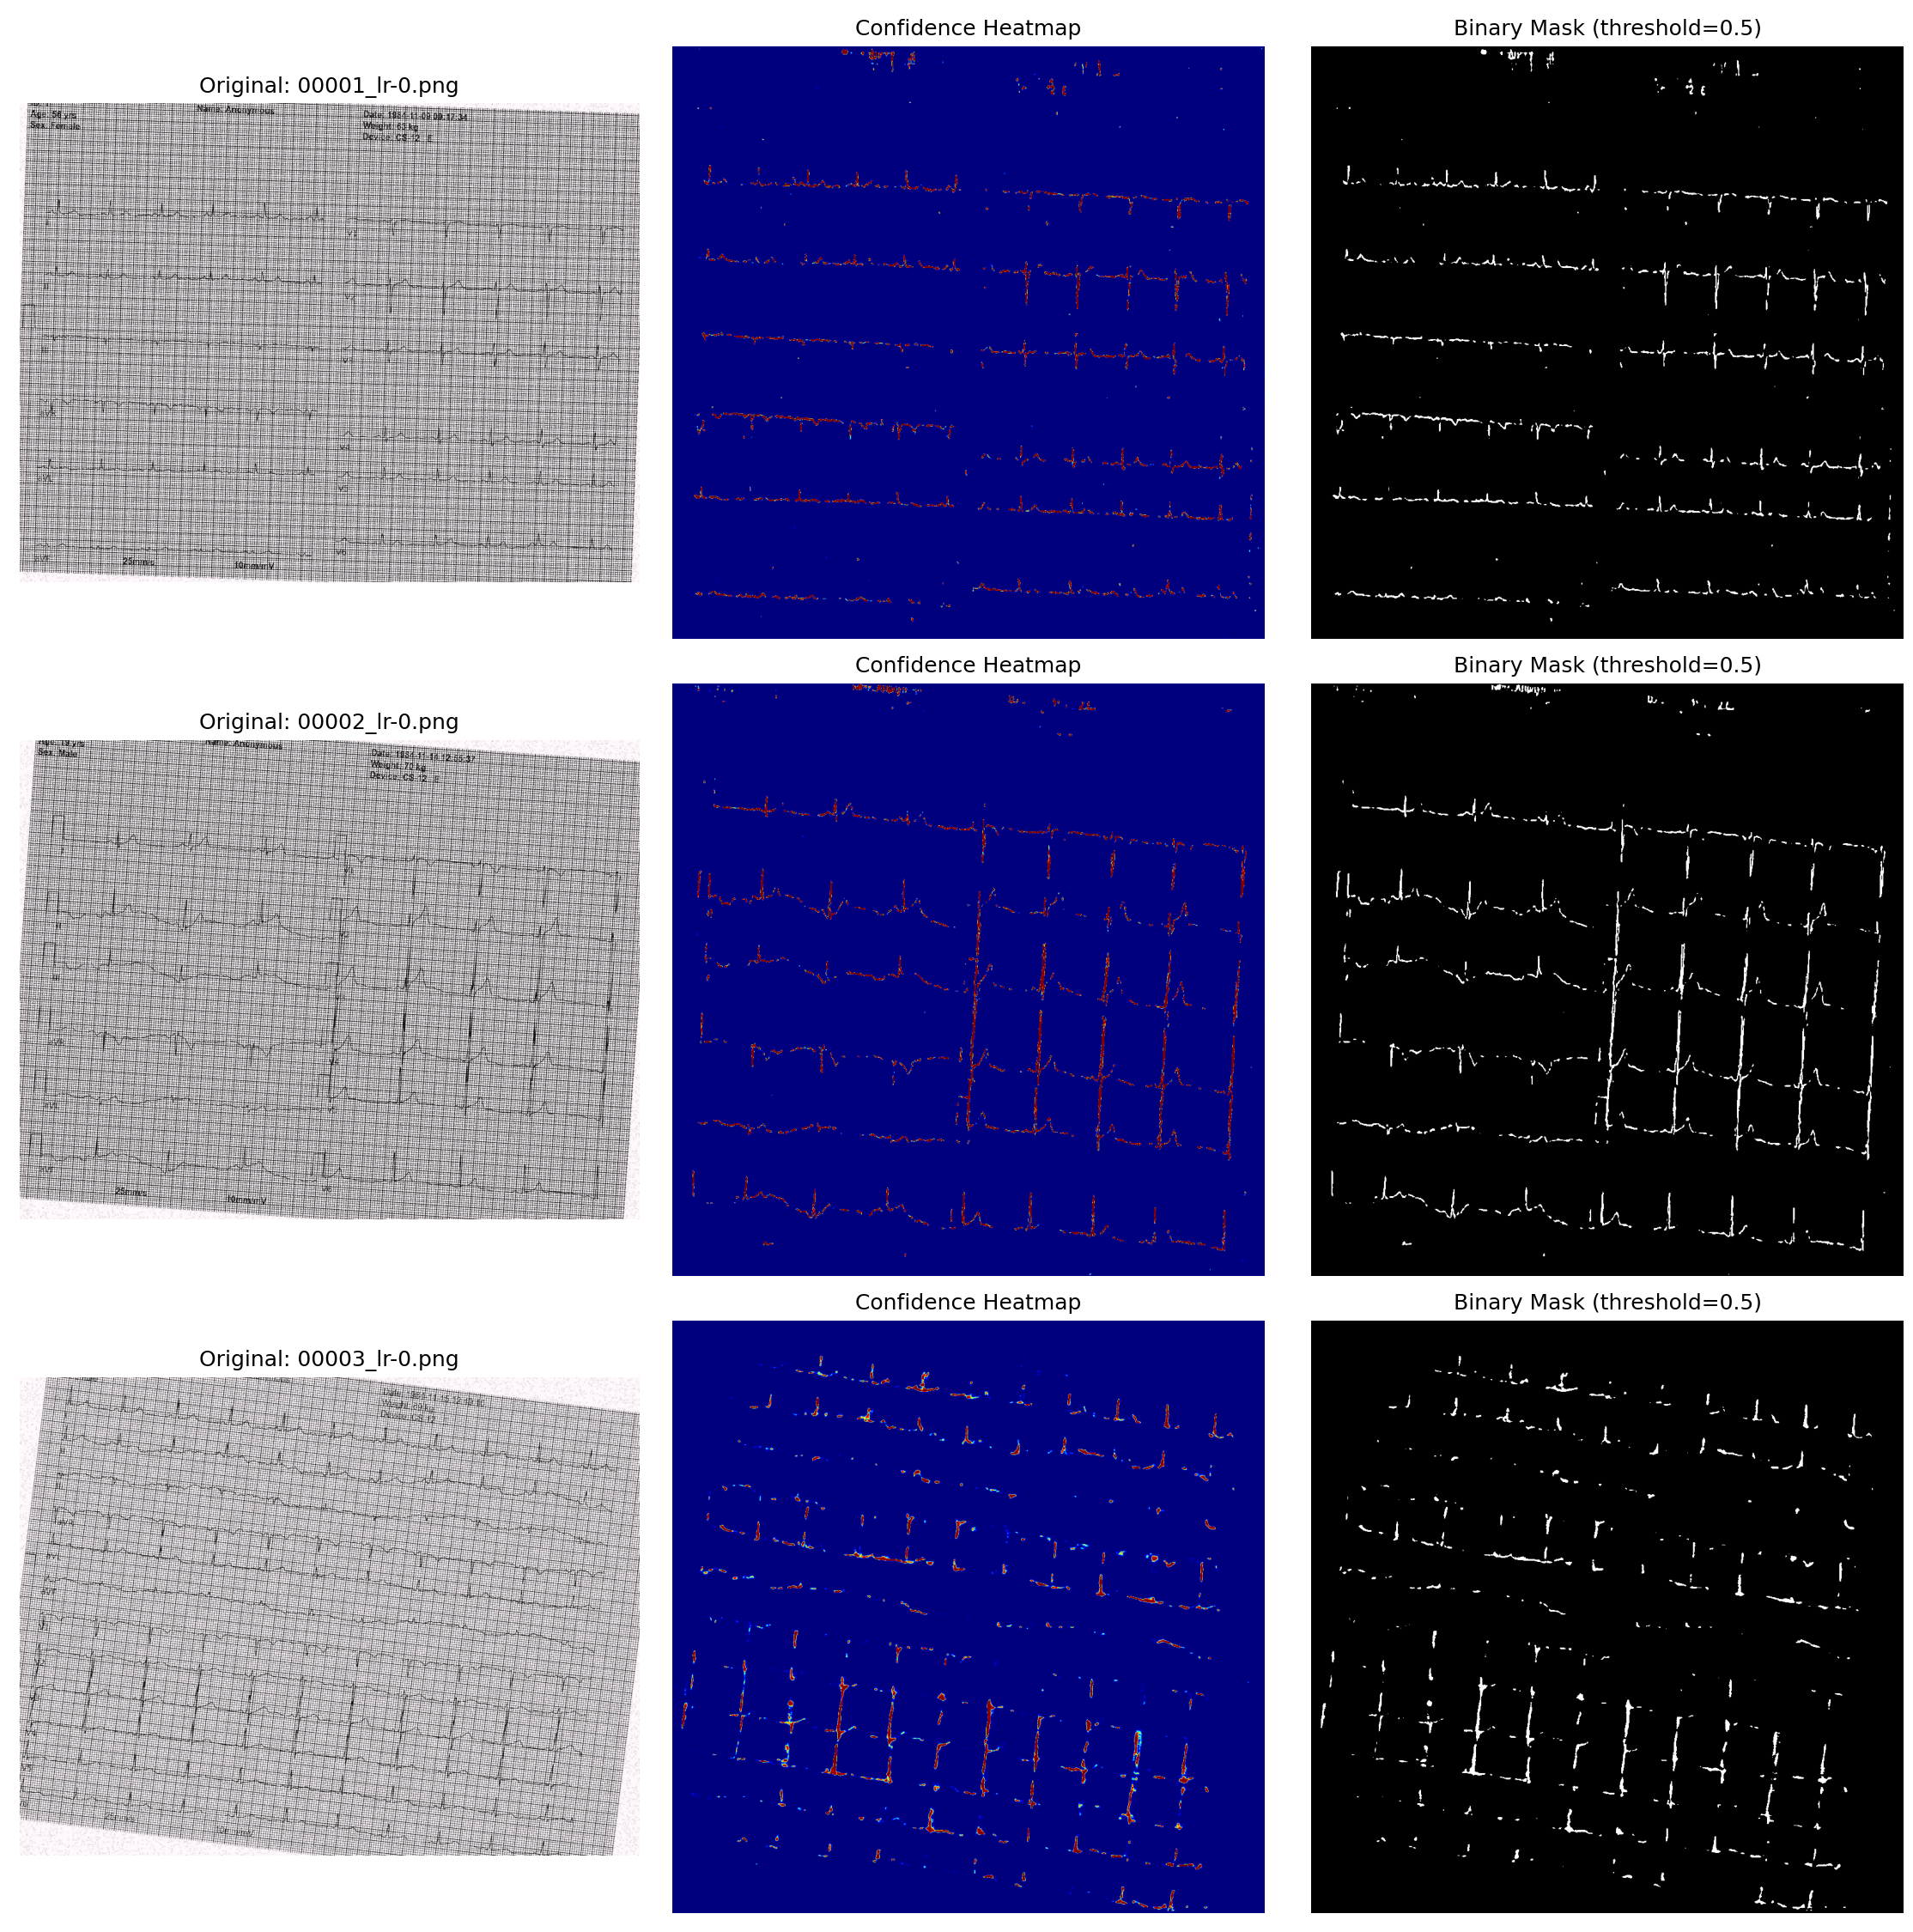
\includegraphics[width=\textwidth,height=4.6cm,keepaspectratio]{viz_seg_stage0.png}\\
      {\scriptsize \texttt{stage0}: heatmap rumorosa, falsi positivi sulla griglia.}
    \end{column}
    \begin{column}{0.5\textwidth}
      \centering
      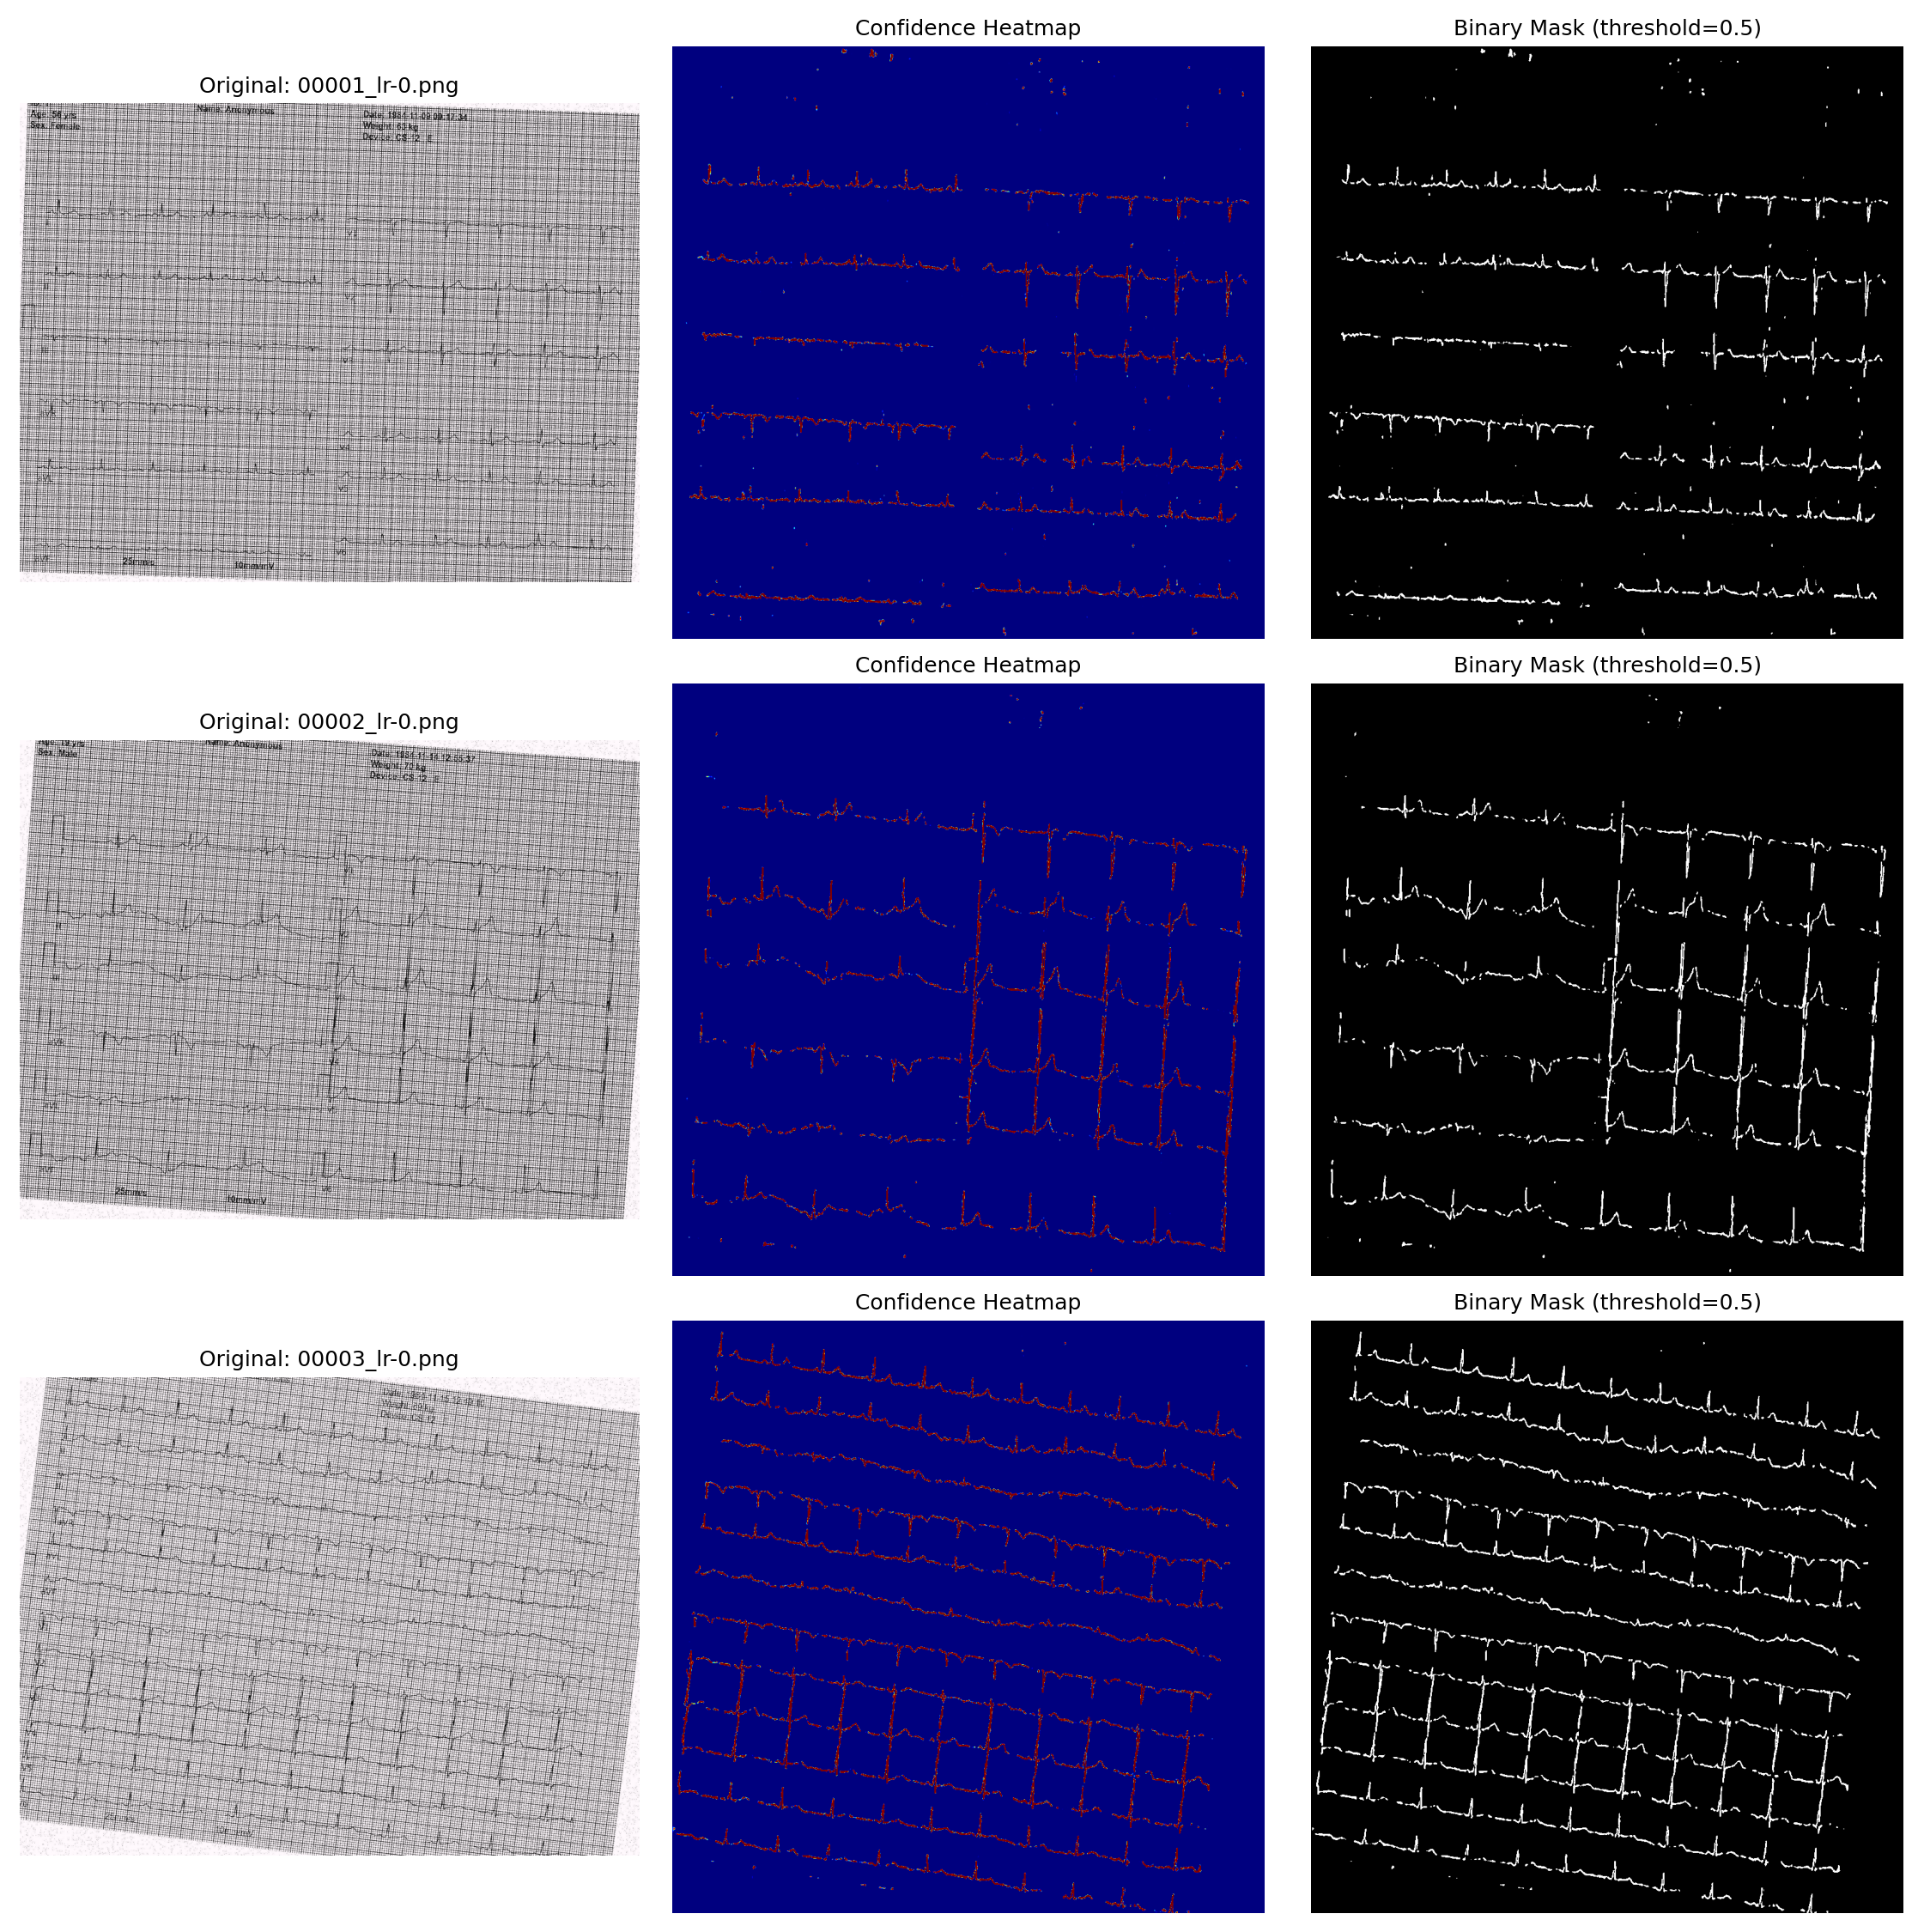
\includegraphics[width=\textwidth,height=4.6cm,keepaspectratio]{viz_seg_stage2.png}\\
      {\scriptsize \texttt{stage2}: maschere più pulite e complete.}
    \end{column}
  \end{columns}
  \vspace{2mm}
  \begin{center}
    Esempi sul \alert{test set sintetico}: il curriculum riduce i falsi positivi sulla griglia e completa i tracciati.
  \end{center}
\end{frame}

\begin{frame}{Estensione: detection head multi-task}
  \begin{columns}[T]
    \begin{column}{0.55\textwidth}
      \begin{itemize}
        \item Oltre alla segmentazione, localizza i \textbf{12 lead}: presenza + bounding box di tracciato ed etichetta.
        \item \alert{Cross-attention per lead}: ogni lead ha una query appresa che seleziona la propria regione.
        \item \textbf{Oriented Bounding Box} (6 parametri, doppio angolo $\sin/\cos 2\theta$) per i tracciati ruotati.
        \item Addestrata in uno stage dedicato a U-Net congelata $\Rightarrow$ nessuna interferenza con la segmentazione.
      \end{itemize}
    \end{column}
    \begin{column}{0.45\textwidth}
      \centering
      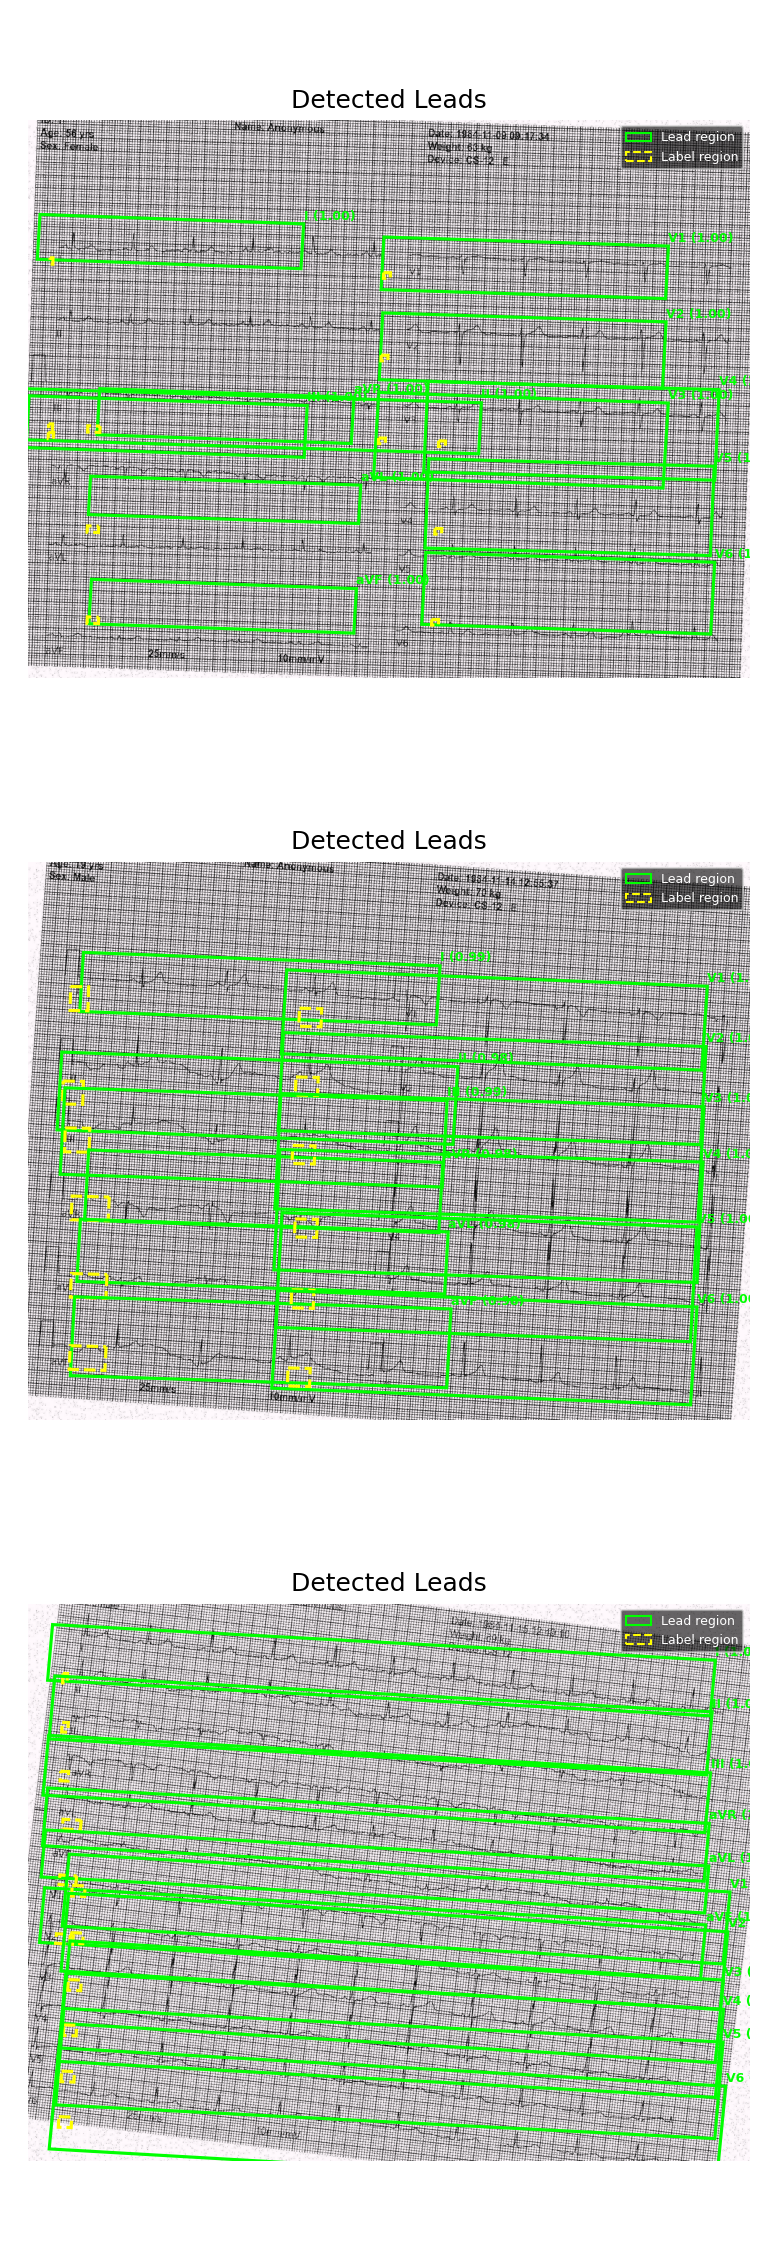
\includegraphics[width=\textwidth,height=5.2cm,keepaspectratio]{viz_det_after.png}\\
      {\scriptsize Lead localizzati: box verdi = tracciato, gialli = etichette.}
    \end{column}
  \end{columns}
\end{frame}

\section{Conclusioni}

\begin{frame}{Conclusioni}
  \begin{block}{Contributi}
    \begin{itemize}
      \item Pipeline di \alert{generazione sintetica} estesa: artefatti realistici, ground truth automatica, parallelizzazione ($3\times$), supporto multi-dataset.
      \item Modello di \alert{segmentazione} U-Net+scSE con loss composita (Focal+Dice+clDice) e curriculum learning a tre stage.
      \item Detection head multi-task con cross-attention e OBB per la localizzazione dei lead.
    \end{itemize}
  \end{block}
  \begin{block}{Sviluppi futuri}
    \begin{itemize}
      \item Conversione \alert{maschera $\rightarrow$ segnale numerico} (digitalizzazione completa).
      \item Validazione estesa su archivi clinici reali.
    \end{itemize}
  \end{block}
\end{frame}

{\setbeamertemplate{footline}{}
\begin{frame}[plain]
  \vfill
  \centering
  {\Huge\color{unitoblue}\textbf{Grazie per l'attenzione}}\\[6mm]
  {\large Matteo Sardi}\\[1mm]
  {\normalsize Generazione Sintetica e Segmentazione di Immagini ECG}\\[6mm]
  
\includegraphics[height=1.4cm,keepaspectratio]{unito_logo.pdf}
  \vfill
\end{frame}}

\end{document}
